\documentclass[twoside]{article}
\usepackage{graphicx}

%\usepackage[latin1]{inputenc}
\usepackage[utf8]{inputenc}
\usepackage[spanish]{babel}
\usepackage{amsmath, amsthm, amsfonts}
\usepackage{textcomp}
\usepackage[T1]{fontenc}
\usepackage{hyperref}
\usepackage{array}
\usepackage{MnSymbol}   % Para poder escribir el cuadrado negro

\usepackage{geometry}
    \geometry{a4paper,total={210mm,297mm},left=35mm,right=30mm,top=30mm,bottom=30mm,}

\usepackage{listings}

\usepackage{tikz}
\usetikzlibrary{arrows,shapes,trees}

\title{\begin{center} 

\includegraphics[scale=0.3]{images/upc.jpg} 
\end{center} 
\vspace{1cm} 
Projecte Final de Carrera\\
ENGINYERIA INDUSTRIAL \\
\vspace{1.5cm} 
\Huge{Control d'un Quadcopter} 
\vspace{2cm} \\ 
Memòria}
%\author{Gabriel de la Cal Mendoza}
\date{}

\usepackage{fancyhdr}		%% Para cabezera de página

\pagestyle{fancy}

% \lhead[x1]{x2}
% \chead[y1]{y2}
% \rhead[LE,RO]{z2}
% \renewcommand{\headrulewidth}{0.5pt}

% \lfoot[a1]{b2}
% \cfoot[c1]{d2}
% \rfoot[LE,RO]{
\includegraphics[scale=0.1]{etseib.jpg}}
% \renewcommand{\footrulewidth}{0.5pt}

\fancyhead[LO,RE]{Quadcopter Control}
\fancyhead[LE,RO]{\thepage}
\fancyfoot[LE,RO]{
\includegraphics[scale=0.1]{images/etseib.jpg}}
\fancyfoot[C]{}

\begin{document}
\maketitle
\begin{center}
\large{
$\begin{array}{ll}
\mbox{Autor:} & \mbox{Gabriel de la Cal Mendoza} \\
\mbox{Director:} & \mbox{Manel Velasco Garcia} \\
\mbox{Convocatòria:} & \mbox{Data a presentar}
\end{array}$}
\\ \vspace{2cm} \Large{Escola Tècnica Superior d'Enginyeria Industrial de Barcelona}\\ \vspace{1cm}

\includegraphics[scale=0.4]{images/etseib.jpg}
\end{center}

\thispagestyle{empty}
\newpage
\begin{center}

\end{center}
\thispagestyle{empty}
\newpage
\setcounter{page}{1}
\section*{Resum}
\newpage
\begin{center}

\end{center}
\thispagestyle{empty}
\newpage

\setcounter{page}{1}
\tableofcontents
\addcontentsline{toc}{section}{Resum}
\fancyhead[LE,RO]{3}
\fancyfoot[C]{}
\newpage
\fancyhead[LE,RO]{\thepage}
\setcounter{page}{4}
\listoffigures
\newpage

\section{Prefaci} 
\subsection{Motivació}

La principal motivació d'aquest projecte és la d'aplicar els coneixements bàsics adquirits en aquests 6 anys de carrera, i més en particular en l'àrea del control en haver fet l'intensificació d'automàtica.\\

Llavors, a l'hora de plantejar un tema per al projecte ràpidament va sorgir la idea de realitzar-lo sobre el control d'un sistema, i més en particular sobre un que estigués actualment emergent tant en mercats com en el camp de l'investigació.\\ 

D'entre les diferents alternatives, un quadcopter és la més atractiva tant per la seva simplicitat constructiva com pel no excessiu cost. Existeixen actualment en el mercat infinitat de proveïdors dels components necessaris per a construïr un quadcopter, amb un gran ventall d'opcions per a escollir cada element com motors, bateries, electrònica, etc.\\

Les possibles aplicacions són nombroses, tant que encara no s'han ni tan sols explotat totes les possibles. Com a exemple: vigilància de superfícies obertes, transport de petits paquets, eina d'oci, entre d'altres.\\

%Com a experiència prèvia es va realitzat el Pre-Projecte sobre quadcopters amb la plataforma open source $ArduPilot$.   

El preu d'un quadcopter no es gaire elevat ja que un comercial com el $AR Drone 2.0$ oscil·la els 300 € i en construïr un amb menys prestacions no hauria de superar aquest cost.

\subsection{Requeriments previs}

Com a requeriments previs és necessari tenir certs coneixements mínims en automàtica per tal de controlar el quadcopter, aíxí com l'inquietut per aprendre el que sigui necessari per a complir, en la mesura del possible, els objectius inicials del present projecte com superar les dificultats que hagin sorgit, tenint en compte que el fi no justifica els medis.
 
\newpage
\section{Introducció}
Un Quadcopter es un vehicle volador no tripulat ($Unmanned Aerial Vehicle$) que es caracteritza per tenir quatre rotors a mode d'actuadors en comptes de dos com en el cas dels helicòpters. Aquest tipus d'autogir intenta obtenir una flotabilitat estable i vol precís balancejant les forces produïdes pels quatre motors. \\

Un dels avantatges que s'obtenen amb aquest canvi és la major capacitat de càrrega ja que es tenen 4 motors  per a soportar el pes. L'estabilitat del vehicle millora en permetre aterratges i enlairaments verticals amb una major maniobrabilitat. També pot treballar en àreas de difícil accés o més agressives, com amb pluja i vent. \\



\subsection{Estudi de l'art}
\subsection{Objectius del projecte}
Esquemàticament es pot representar com una estructura en $X$ amb el seu centre coincidint amb el centre de masses i quatre actuadors a les puntes de cada braç, tots ells apuntant en la mateixa direcció y sentit

descripción por encima\\
historia\\
estudio del arte\\
futuras aplicaciones\\

% \section{Estudi de l'art}
\newpage
\section{Definicio del model}
\subsection{Definició de les variables}
Per a caracteritzar la planta amb la que es treballarà, és necessari obtenir un model del quadcopter. Les constants pròpies del model es deixaran en forma de paràmetres a calibrar una vegada es tingui l'objecte físic. D'aquesta manera el model serà general per a tot quadcopter que comparteixi la mateixa família de paràmetres.
És necessari considerar dos marcs de referència: l'inercial format pels eixos $x,y,z$ i el del cos (Body) format pels eixos $x_B,y_B,z_B$. El primer té la persepectiva de l'observador en terra, estàtic, mentre que el segon és solidari a l'estructura. Segons l'orientació del eixos del cos amb aquesta referència es poden donar els següents dos cassos:
\begin{itemize}
\item $Cross type$: Els eixos de coordenades coincideixen amb els braços de l'estructura ja que es tenen els actuadors a les puntes de cada braç.
\item $X-type$: Els eixos i l'estructura formen 45º. Es tenen llavors dos motors al davant i dos al darrere.
\end{itemize} 
Per ser més usual la primera opció, es decideix utilitzar la configuració $Cross type$ tal i com es té en la figura \ref{RefQuad}.
\begin{figure}[h!]
\centering
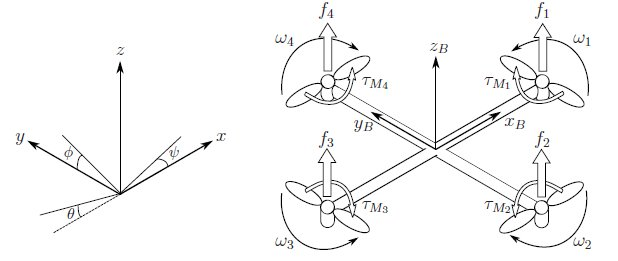
\includegraphics[scale=0.5]{images/quad.jpg}
\caption{Marcs de referència en el quadcopter}
\label{RefQuad}
\end{figure}\\
Es suposa que l'objecte és un rotor esfèric, i per tant el seu tensor d'inèrcia és diagonal:
\begin{equation}I=\left[ \begin{array}{ccc}
I_{xx} & 0 & 0 \\
0 & I_{yy} & 0 \\
0 & 0 & I_{zz} 
\end{array} \right] \end{equation}
Es defineix la posició linear absoluta amb les coordenades $x,y,z$ pel vector $\xi$ i igualment per a la posició angular a partir de $\eta$ segons:
\begin{equation}
\xi=\left[ \begin{array}{ccc}
x\\
y\\
z \end{array} \right] ,\quad \eta=\left[ \begin{array}{ccc}
\phi\\
\theta\\
\psi \end{array} \right] , \quad q=\left[\begin{array}{c}
\xi\\
\eta \end{array} \right] 
\end{equation}

on $\phi$ és l'angle de capcineig (Pitch), $\theta$ és el de balanceig (Roll) i $\psi$ el de guiñada (Yaw).\\
Per a l'orientació angular entre els dos marcs es té un sistema de referència amb angles Tait Bryan, on la matriu de transformació és:
\begin{equation}
R=\left[\begin{array}{ccc}
C_\psi C_\theta & C_\psi S_\theta S_\phi - S_\psi C_\phi & C_\psi S_\theta C_\phi + S_\psi S_\phi \\
S_\psi C_\theta & S_\psi S_\theta S_\phi + C_\psi C_\phi & S_\psi S_\theta C_\phi - C_\psi C_\phi \\
-S_\theta & C_\theta C_\phi & C_\theta C_\phi 
\end{array}\right]
\end{equation}
amb $C_\phi=cos(\phi)$ i $S_\phi=sin(\phi)$.\newpage
Les velocitats lineals en el marc de referència del cos (Body Frame) es representen amb el vector $v_B$ y les velocitats angulars amb $\gamma$ segons:
\begin{equation}
v_B=\left[\begin{array}{c}
v_{x,b}\\
v_{y,b}\\
v_{z,b}\\
\end{array}\right] \hspace{1cm} \gamma=\left[\begin{array}{c}
p\\
n\\
r
\end{array} \right]
\end{equation}
En canvi, les velocitats en el marc de referència inercial (Inertial Frame)  es representen per $\dot{\eta}$ per a les velocitats lineals i per $\dot{\xi}$ per a les angulars: 
\begin{equation}
\dot{\xi}=\left[\begin{array}{c}
\dot{x} \\
\dot{y} \\
\dot{z}
\end{array} \right] \hspace{1cm} \dot{\eta}=\left[\begin{array}{c}
\dot{\psi} \\
\dot{\theta} \\
\dot{\psi}
\end{array} \right] 
\end{equation}
Ja que la derivada dels angles $\phi$, $\theta$ i $\psi$ no és el vector de velocitats angulars és necessari tenir un canvi de base per relacionar el marc de referència inercial al del cos amb la matriu $W_\eta$:
\begin{equation}
W_\eta=\left[\begin{array}{ccc}
1 & 0 & -S_\theta \\
0 & C_\phi & C_\theta S_\phi \\
0 & -S_\phi & C_\theta C_\phi 
\end{array} \right] \hspace{0.5cm} amb \hspace{0.5cm} 
\gamma=\left[ W_\eta \right] \dot{\eta} 
\end{equation}
Les forces de sustentació i moments generats pels quatre actuadors són $f_1,f_2,f_3,f_4$ i $w_1,w_2,w_3,w_4$ respectivament. Seguint l'orientació de la figura \ref{RefQuad}, per tal de poder anular els moments produïts en l'eix $z_B$ (en el marc del cos) el sentit de gir dels actuadors  $4$ i $2$ és en el de les agulles del rellotge (clockwise) i els dels $1$ i $3$ en sentit contrari (counterclockwise). \\

Interessa conèixer quina força i moment aportarà cada motor per a una velocitat angular coneguda. Es tenen les següents relacions per a cada actuador: 
\begin{equation}
\begin{array}{l}
f_i=kw^2_i \\ 
\tau_{M_i}=bw^2_i
\end{array}
\end{equation}
Per tant l'empenta total $T_B$ proporcionada en la direcció $z_B$ i els moments generats $\tau_B$ pels motors és:
\begin{equation}
T_B=k\left(\sum_{i=1}^{4}w^2_i \right)e_{z_B}=\left[ \begin{array}{c}
0 \\
0 \\
\displaystyle\sum_{i=1}^{4}w^2_i
\end{array} \right] 
\hspace{1cm} \tau_B=\left[ \begin{array}{c}
\tau_\phi \\
\tau_\theta \\
\tau_\psi
\end{array} \right] = \left[ \begin{array}{c}
lk(w^2_4 - w^2_2) \\
lk(w^2_3 - w^2_1) \\
\displaystyle\sum_{i=1}^{4}\tau_{M_i}
\end{array} \right]
\end{equation}

\subsection{Obtenció del model}
Les equacions que governen el sistema s'obtenen amb el mètode de Euler-Lagrange, pel que es parteix obtenint el Lagrangià del sistema:
\begin{equation}
\mathcal{L}=E_{cinetica} - E_{potencial} = (E_{translacio}+E_{rotacio})-E_{potencial}
\end{equation}

Substituïnt cada component per la seva expressió:
\begin{equation}
\mathcal{L}(q,\dot{q})=\frac{m}{2} \dot{\xi}^T \dot{\xi} + \frac{1}{2}\gamma^{T}I\gamma - mgz
\end{equation}
Es troba el vector de forçes i moments com:
\begin{equation}
F=\left[ \begin{array}{c}
f \\
\tau_B
\end{array} \right] = \frac{d}{dt}\left(\frac{\partial \mathcal{L}}{\partial \dot{q}}\right)-\frac{\partial\mathcal{L}}{\partial q}
\end{equation}

amb $ \hspace{0.5cm} q=[\begin{array}{cccccc}
x & y & z & \phi & \theta & \psi
\end{array} ]^{T} \hspace{0.5cm}$ i $ \hspace{0.5cm} \dot{q}=[\begin{array}{cccccc}
\dot{x} & \dot{y} & \dot{z} & \dot{\phi} & \dot{\theta} & \dot{\psi}
\end{array} ]^{T}$.\\

En calcular $F$ és necessari fer el canvi de variables de $\gamma$ a $\dot{\eta}$ amb el canvi de base $\dot{\eta}=\left[ W_\eta \right]^{-1} \gamma$ per tal de poder derivar el Lagrangià respecte $\dot{q}$, que són les variables pròpies del marc de referència inercial

\begin{equation}
\frac{1}{2}\gamma^{T}I\gamma = \frac{1}{2}(W_\eta \dot{\eta})^{T}I(W_\eta \dot{\eta}) = \frac{1}{2}\dot{\eta}^{T}(W_\eta ^{T}IW_\eta)\dot{\eta} = \frac{1}{2}\dot{\eta}^{T}J\dot{\eta}
\end{equation}

on la matriu $J$ queda com
\begin{equation}
J=W_\eta ^{T}IW_\eta = \left[ \begin{array}{ccc}
I_{xx} & 0 & -I_{xx} S_\theta \\
0 & I_{yy} C^2_\phi + I_{zz} S^2_\phi & (I_{yy}-I_{zz}) C_{\phi} S_\phi C_\theta \\
-I_{xx} S_\theta & (I_{yy}-I_{zz}) C_{\phi} S_\phi C_\theta & I_{xx} S^2_{\theta}+I_{yy} S^2_{\phi} C^2_\theta +I_{zz}C^2_{\phi} C^2_{\theta}
\end{array} \right]
\end{equation} 

i per tant el Lagrangià queda com:

\begin{equation}
\mathcal{L}(q,\dot{q})=\frac{m}{2} \dot{\xi}^T \dot{\xi} + \frac{1}{2}\dot{\eta}^{T}J\dot{\eta}- mgz
\end{equation}
Les components lineals y angulars no depenen unes de les altres, i per tant es poden estudiar per separat obtenint dos equacions: una per les forces lineals y un altre per als moments. Això vol dir que la força que exerceixen els actuadors no depenen de les velocitats angulars que es tinguéssin, i tampoc es tindran accel·leracions angulars diferents segons l'altura a la que es trobi el quadcopter: l'objecte girarà de la mateixa manera sigui quina sigui la seva posició en l'espai.

Llavors, fent la derivada parcial respecte $\dot{q}$ s'obté
\begin{equation}
 F=\frac{d}{dt}\left(\frac{m}{2}(1\cdot\dot{\xi}+\dot{\xi}\cdot 1)+\frac{1}{2}\frac{\partial}{\partial \dot{\eta}}(\dot{\eta}^{T}J\dot{\eta})\right)-\frac{\partial \mathcal{L}}{\partial q}
\end{equation}

Com que $J$ és una matriux simètrica, es pot dir que  $\frac{\partial}{\partial \dot{\eta}}(\dot{\eta}^{T}J\dot{\eta})=2 \frac{\partial}{\partial \dot{\eta}}(\dot{\eta}^{T}J)\dot{\eta} $. \\

\textbf{Demostració:} Per probar això es veurà per al cas $\frac{\partial}{\partial x}(x^{T}Ax)=2 \frac{\partial}{\partial x}(x^{T}A)x $ amb 

\begin{equation}
x=\left[ \begin{array}{c}
x_1 \\
x_2 \\
x_3 
\end{array} \right] \hspace{1cm} A=\left[ \begin{array}{ccc}
a_{11} & a_{12} & a_{13} \\
a_{21} & a_{22} & a_{23} \\
a_{31} & a_{32} & a_{33} 
\end{array} \right]
\end{equation}
Llavors
\begin{equation}
\frac{\partial}{\partial x}(x^{T}A x) = \frac{\partial}{\partial x}\left(\left[x_1 x_2 x_3 \right]\left[\begin{array}{ccc}
a_{11} & a_{12} & a_{13} \\
a_{21} & a_{22} & a_{23} \\
a_{31} & a_{32} & a_{33} 
\end{array} \right]\left[\begin{array}{c}
x_1 \\
x_2 \\
x_3 
\end{array} \right] \right) =
\end{equation}
\begin{equation}
\frac{\partial}{\partial x}(x^2_1 a_{11}+x_1x_2a_{21}+x_1x_3a_{31} + x_1x_2a_{12}+x^2_xa_{22}+x_2x_3a_{32} + x_1x_3a_{13}+x_2x_3a_{23}+x^2_3a_{33})=
\end{equation}
Com que $A$ és simètrica $a_{12}=a_{21}$, $a_{13}=a_{31}$ i $a_{23}=a_{32}$, i en fer la derivada direccional resulta
\begin{equation}
\frac{\partial}{\partial x}(x^{T}A x)=\left[ \begin{array}{c}
2x_1a_{11}+x_2a_{21}+x_3a_{31}+x_2a_{12}+x_3a_{13} \\
x_1a_{21}+x_1a_{12}+2x_2a_{22}+x_3a_{32}+x_3a_{23} \\
x_1a_{31}+x_2a_{32}+x_1a_{31}+x_2a_{23}+2x_3a_{23}
\end{array} \right]=2\cdot\left[ \begin{array}{c}
x_1a_{11}+x_2a_{12}+x_3a_{13} \\
x_1a_{12}+x_2a_{22}+x_3a_{23} \\
x_1a_{13}+x_2a_{23}+x_3a_{23}
\end{array} \right]
\end{equation}
I en avaluar l'altre costat de la igualtat es té el mateix resultat
\begin{equation}
2 \frac{\partial}{\partial x}(x^{T}A)x=2 \frac{\partial}{\partial x} \left( \left[ \begin{array}{ccc}
x_1a_{11}+x_2a_{12}+x_3a_{13} \\
x_1a_{21}+x_2a_{22}+x_3a_{23} \\
x_1a_{13}+x_2a_{32}+x_3a_{33}
\end{array} \right]^{T} \right)x=
\end{equation}
\begin{equation}
=2\left[\begin{array}{ccc}
a_{11} & a_{12} & a_{13} \\
a_{21} & a_{22} & a_{23} \\
a_{31} & a_{32} & a_{33} 
\end{array} \right]\cdot\left[\begin{array}{c}
x_1 \\
x_2 \\
x_3
\end{array} \right]=2\cdot\left[ \begin{array}{c}
x_1a_{11}+x_2a_{12}+x_3a_{13} \\
x_1a_{12}+x_2a_{22}+x_3a_{23} \\
x_1a_{13}+x_2a_{23}+x_3a_{23}
\end{array} \right]
\end{equation}
\hfill $\blacksquare$ \newpage
Com que $2 \frac{\partial}{\partial \dot{\eta}}(\dot{\eta}^{T}J)\dot{\eta}=2 J \dot{\eta}$ es té, aplicant la regla de la cadena en el producte $J\dot{\eta}$:
\begin{equation}
F=\frac{d}{dt}\left(m \dot{\xi}+J \dot{\eta}\right)-\frac{\partial \mathcal{L}}{\partial q} =m\ddot{\xi} + J\ddot{\eta} + \dot{J}\dot{\eta}-\left( \frac{1}{2} 2 \frac{\partial}{\partial \dot{\eta}} ( \dot{\eta}^{T}J)\dot{\eta} - mg\left[\begin{array}{c}
0 \\
0 \\
1
\end{array} \right] \right)
\end{equation}

Per arribar a aquest resultat s'ha aplicat la derivada direccional a $mgz$:
\begin{equation}
D_q(mgz)=D_\xi(mgz)=mg \left[ \begin{array}{c}
0 \\
0 \\
1
\end{array} \right]
\end{equation}

Separant les components lineals i angulars en dues equacions:
% \begin{equation}
\begin{align}
f & = m \ddot{\xi} + mg \left[ \begin{array}{c}
0 \\
0 \\
1
\end{array} \right] =RT_B\\
\tau & =J \ddot{\eta} +  \underbrace{\left( \dot{J} - \frac{\partial}{\partial \dot{\eta}}(\dot{\eta}^{T}J)\right)}_{C(\eta,\dot{\eta})} \dot{\eta} =J \ddot{\eta} +  C(\eta,\dot{\eta})\dot{\eta} 
\end{align}
% \end{equation}

On $C(\eta,\dot{\eta})$ és la matriu de Coriolis. 
Per obtenir el sistema d'equacions del model s'han d'aïllar les accel·leracions, i s'obté:
\begin{equation}
\begin{cases}
\ddot{\xi} & =\frac{1}{m}RT_{B} - g \cdot \left[ \begin{array}{ccc}
0 & 0 & 1\\
\end{array} \right]^{T} \\
\ddot{\eta} & =J^{-1} \left( \tau - C(\eta,\dot{\eta})\dot{\eta}  \right)
\end{cases}
\label{eq:system}
\end{equation}

Per a realitzar el control será útil representar el sistema \ref{eq:system} en forma d'espai d'estats:

\begin{equation}
\frac{\partial}{\partial t}\left[ \begin{array}{l}
\xi \\
\dot{\xi} \\
\eta \\
\dot{\eta} 
\end{array} \right] =\left[ \begin{array}{l}
\dot{\xi} \\
\frac{1}{m}RT_{B} - g \cdot \left[ \begin{array}{ccc}
0 & 0 & 1 \\
\end{array} \right]^{T} \\
\dot{\eta} \\
J^{-1} \left( \tau - C(\eta,\dot{\eta})\dot{\eta} \right)
\end{array} \right]
\end{equation}

\subsection{Representació del model amb Matlab}





\newpage
\section{Disseny del controlador}
% Explicar que se quiere controlar el Quadcopter mediante la Linealización extendida, trabajando alrededor de puntos de equilibrio
% \Linealització extesa
% Explicar el concepto de Linealización extendida 
% Explicar el proceso de obtención del lagrangiano con el .m,  vector de fuerzas, obtención del sistema linealizado alrededor del punto de equilibrio, observador lineal,... 
\newpage
\section{Implementació del control} 
% Pufff

\newpage
\section{Construcció del Quadcopter}
% Descripción de cómo se hará en general
El conjunt de peces que formen aquest aparell estan conectades entre sí segons la funció que realitzen. Esencialment la Raspberry Pi controla els motors segons les señals que reb de l'IMU i el Receptor. Tot el conjunt és alimentat per una bateria LiPo i s'adapta el voltatge de 11.1V a 5V per mitjà d'un Regulador per tal d'alimentar a la Raspberry. Tots els components estan subjectats a una estructura (Frame) que també pateix les forces y moments.  

\subsection{Descripció dels components}
% Descripción y explicación de cada componente del Quadcopter, con imágenes de cada
Es descriu tot seguit cada component i el criteri de sel·lecció que s'ha aplicat.
\subsubsection*{Raspberry Pi} 
Abreujat com a RPi, és un petit ordinador integrat en una sola placa (Single-Board Computer o SBC en anglès) del tamany d'una targeta de crèdit, és a dir, amb unes dimensions de 85.6cm x 53.98cm, desenvolupat per la Fundació Raspberry Pi amb l'intenció de promocionar les ciències computacionals a les escoles \cite{RPiWiki}. 

%\begin{tabular}{cc}
\begin{figure}[h!]
\begin{center}
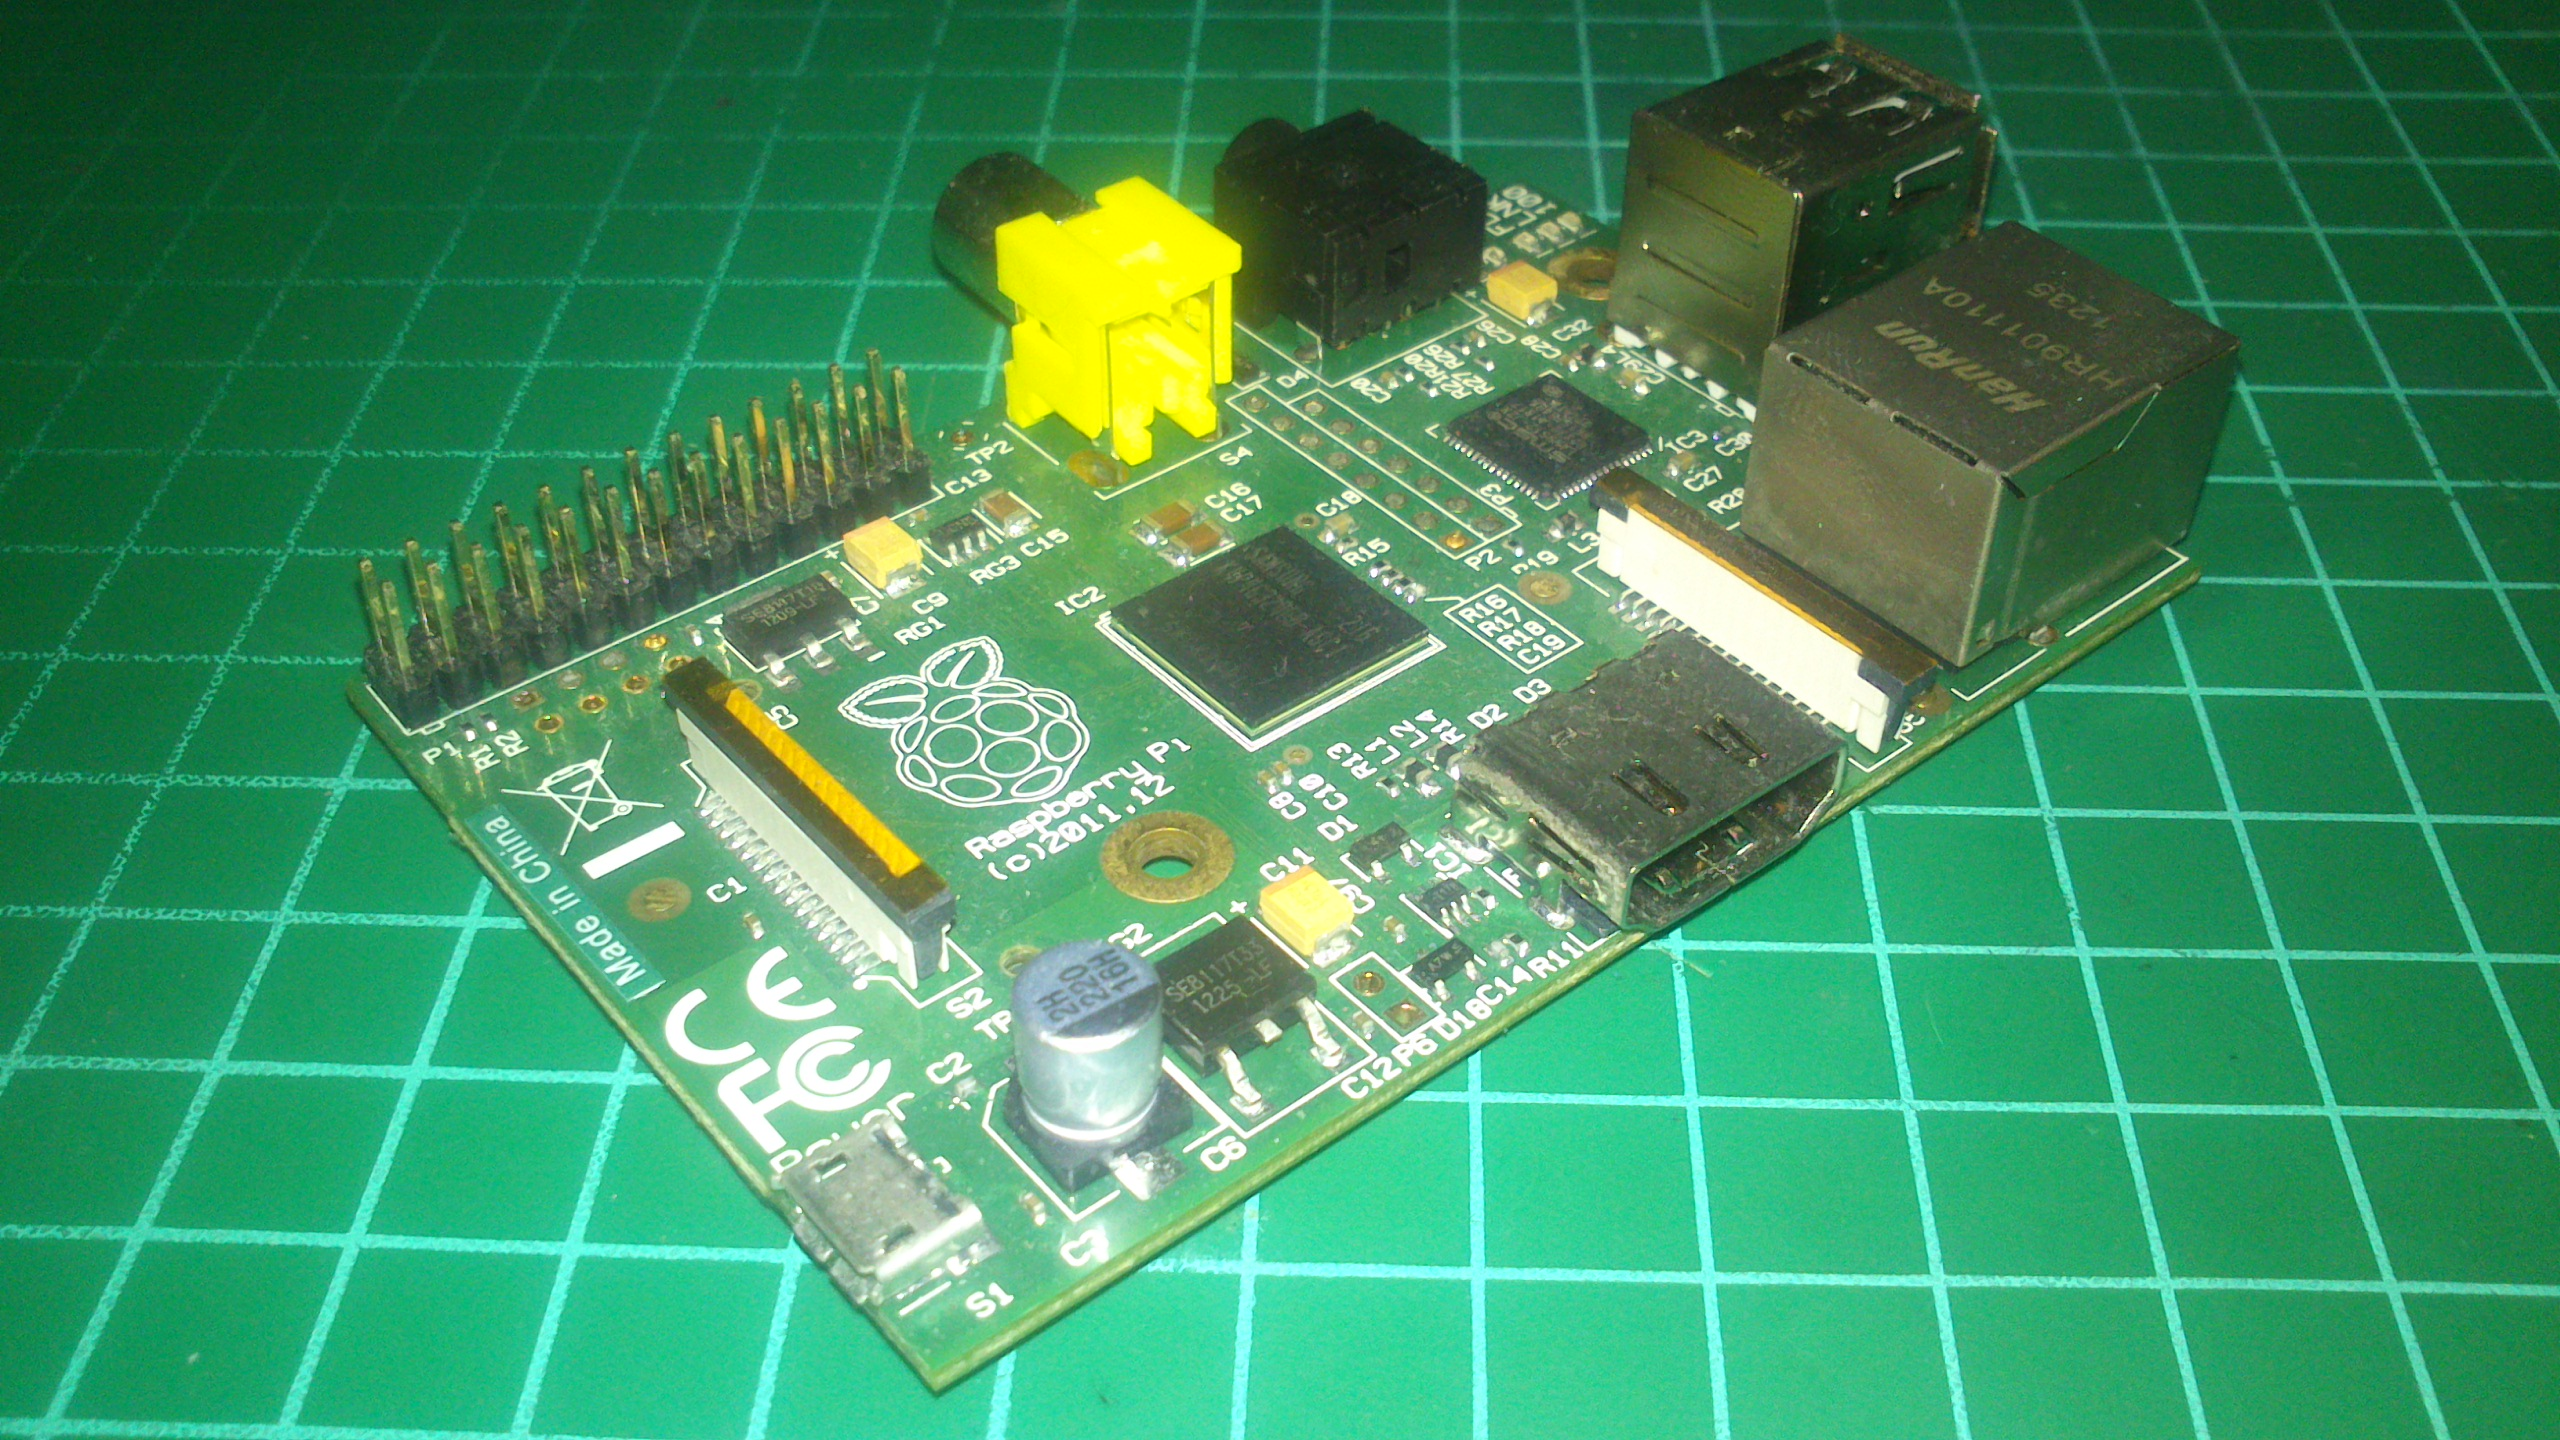
\includegraphics[scale=0.06]{images/RPi.jpg}
\caption{Raspberry Pi a utilitzar}
\label{RPiImage}
\end{center}
\end{figure}
%\end{tabular}

S'ha optat per aquesta opció pel seu econòmic preu, la velocitat de processament i baix consum. A més, s'ha volgut ampliar els coneixements d'aquest petit monstre. En particular s'utilitza la segona revisió del model B:

\begin{figure}[h!]
\begin{center}
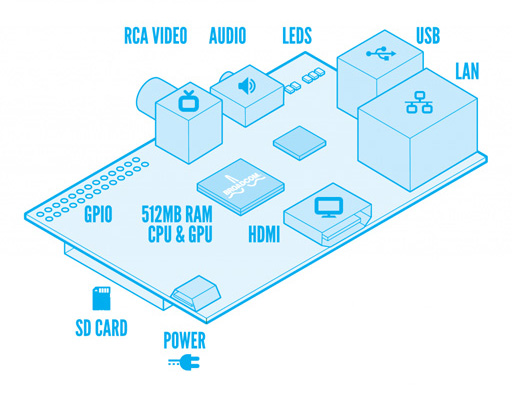
\includegraphics[scale=0.3]{images/RPi2.jpg}
\caption{Conectors de la Raspberry Pi}
\label{RPiConn}
\end{center}
\end{figure}

%\begin{tabular}{cc}
%\hspace{1cm}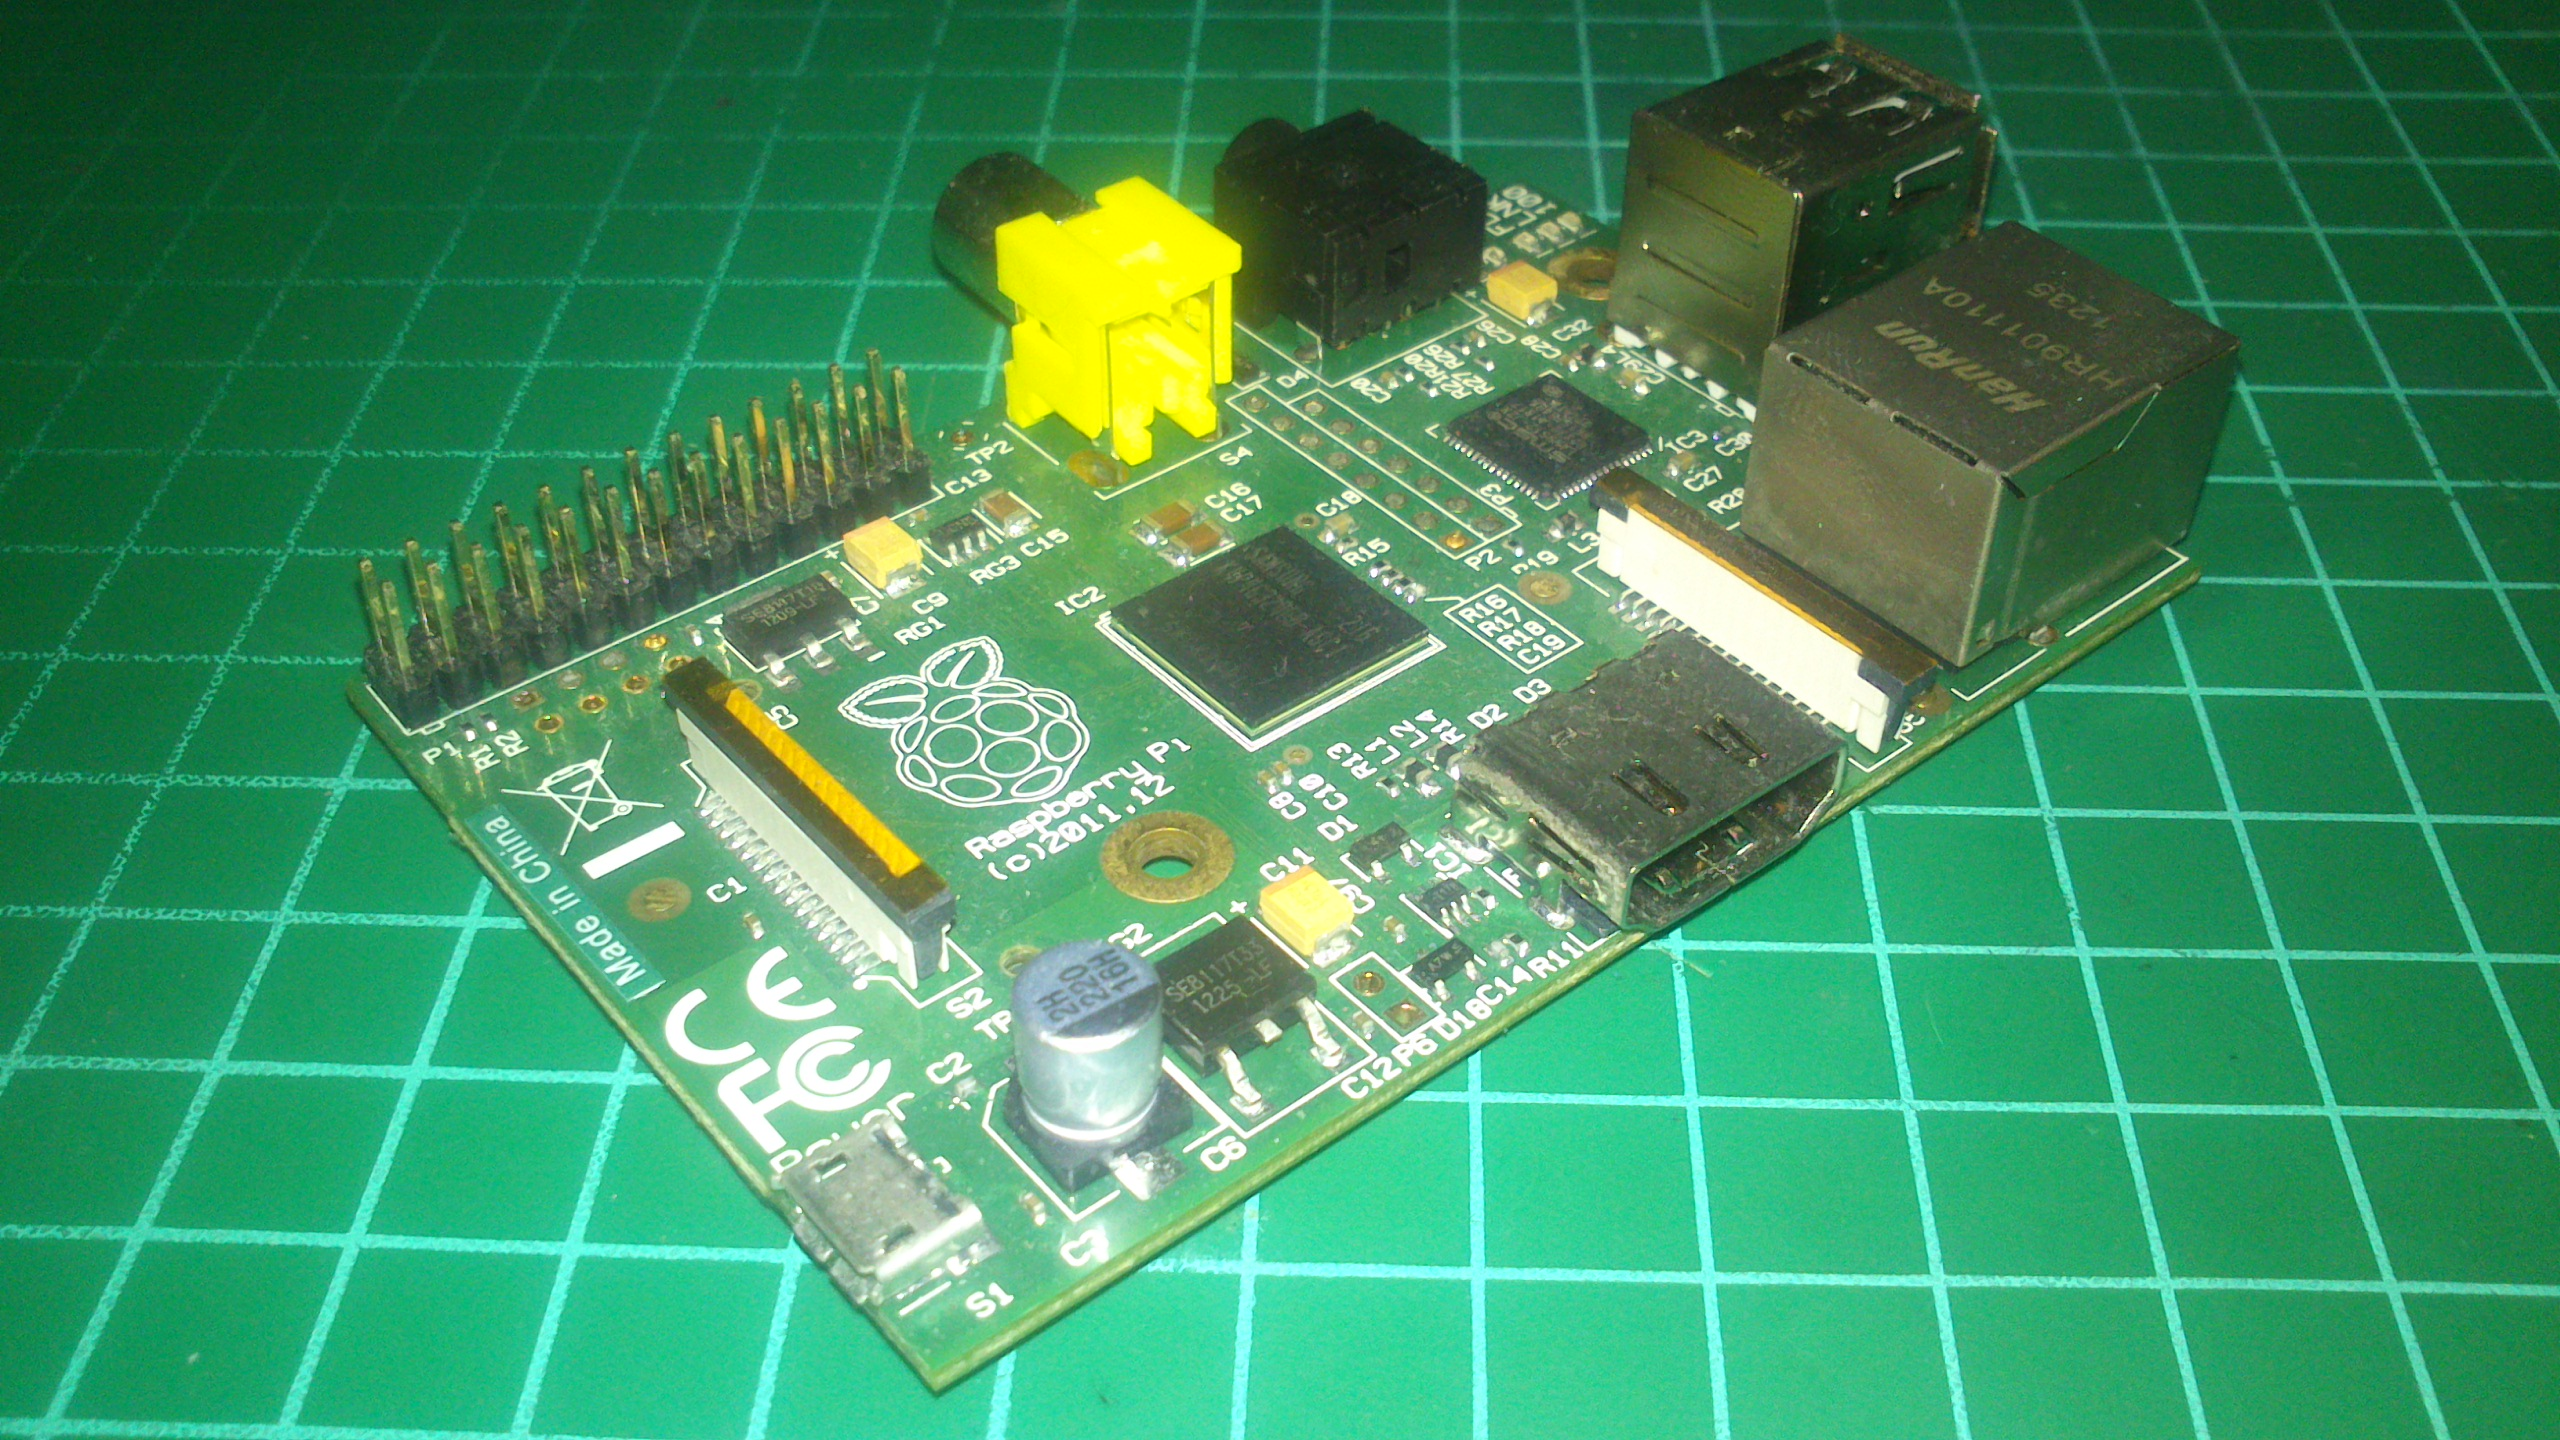
\includegraphics[scale=0.06]{images/RPi.jpg}
%& \hspace{0.5cm} 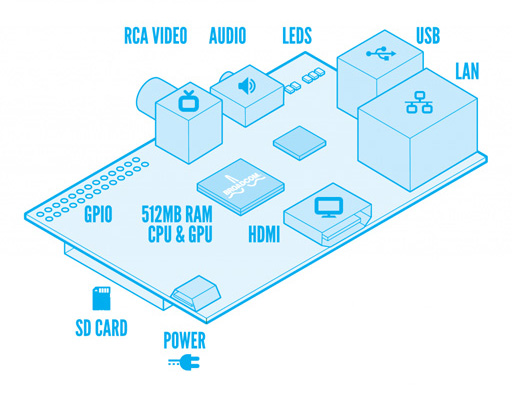
\includegraphics[scale=0.3]{images/RPi2.jpg}
%\end{tabular} \\

Té un System-on-Chip (SoC) Broadcom BCM2835 amb un ARM1176JZF-S a 700 Mhz, una GPU VideoCore IV i 512 MB de memòria RAM. Disposa de dos ports USB, una sortida mini-jack 3.5mm, sortida d'audio/vídeo HDMI, una sortida RCA i un port RJ45 10/100 d'Ethernet. 

L'alimentació es realitza per mitjà d'un mini USB a 5V/700mA, amb un consum de 3.5W. El sistema operatiu és un Raspbian, gravat en una targeta SD de 4GB. Disposa d'un conjunt de pins que permeten comunicació amb perifèrics de baix nivell UART, I2C, SPI i 8 pins de propòsit general (General Porpouse Input Output o GPIO).

\subsubsection*{GY-521 MPU-6050}
Es tracta d'una Unitat de Mesura Inercial (IMU en anglès) que integra en un mateix encapsulat de $4x4x0.9mm$ un acceleròmetre i un giròscop, ambdós de 3 eixos. Disposa dun conversor ADC de 16 bits per a cada eix i es comunica mitjançant un protocol de comunicació $I2C$. S'ha optat per utilitzar aquest dispositiu pel seu baix cost i la fàcil comunicació que comporta amb la RPi.
\begin{figure}[h!]
\begin{center}
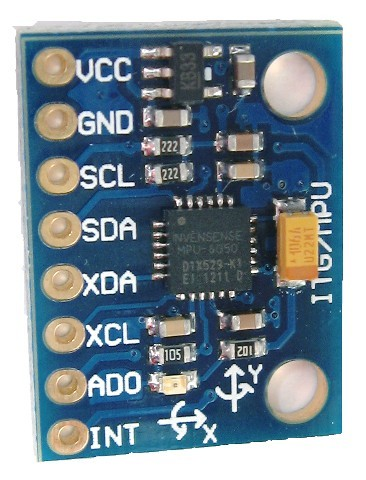
\includegraphics[scale=0.12]{images/mpu-6050.jpg} 
\caption{IMU MPU-6050}
\end{center}
\end{figure}\\
Com a característiques dels sensors: el giròscop té un rang de  $\pm250,\pm500,\pm1000,\pm2000$ graus/segon, i l'accel·leròmetre de $\pm2g,\pm4g,\pm8g,16g$. La tensió d'alimentació és del rang de $2.375V-3.46V$ i cap la possibilitat d'utilitzar un mòdul $DMP$ (Digital Motion Processor), però s'ha decidit implementar un filtre de Kalman per llegint les dades en cru (raw) de la cua $FIFO$ del sensor.

\subsubsection*{Emissor-Receptor}
Amb aquest parell de components es transmet la consigna generada des del transmissor cap al receptor mitjançant ones de radio. El model que s'utilitza és el $Turnigy 5X 5Ch Mini$, per què és un model fàcil d'utilitzar i econòmic. Les especificacions tècniques més rellevants són: 

\begin{figure}[h!]
\begin{center}
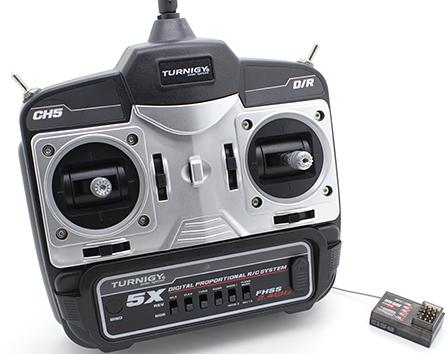
\includegraphics[scale=0.4]{images/E_R.jpg} 
\caption{Emissora i Receptor}
\end{center}
\end{figure}

El transmissor té unes dimensions de $156x152x50mm$, un pes de 265g i s'alimenta a 6V (4 bateries AA). El receptor té unes mides de $33.5x20.5x13mm$ i s'alimenta a 4.8-6V. Disposa de 5 canals de radio, amb transmissió segura a 2.4GHz amb el mètode FHSS. Pot configurarse per traballar amb dos modes (mode1-mode2).

La senyal que es reb per cada canal en el receptor és de $PWM$ de $50Hz$ amb un Duty que veria de $1ms$ a $2ms$.

%% Especificación por canal de los PWM: mínimo y máximo Duty
%% Mirar con osciloscopio la señal

\subsubsection*{Bateria LiPo}
Per a alimentar a tot el conjunt s'utilitza una LiPo $Turnigy 2200mAh 3S1P 25C$. Per tant, és capaç d'entregar 2.2A durant una hora, i com que la capacitat és de 25C, la descàrrega pot ser de $2.2*25=55A$ amb un pic de descàrrega de 35C, és a dir, amb un pic de $2.2*35=77A$ durant 10 segons. Aquesta bateria està formada per tres cel·les que proporcionen un voltatge total d'uns $11.1V$:\\
\begin{center}
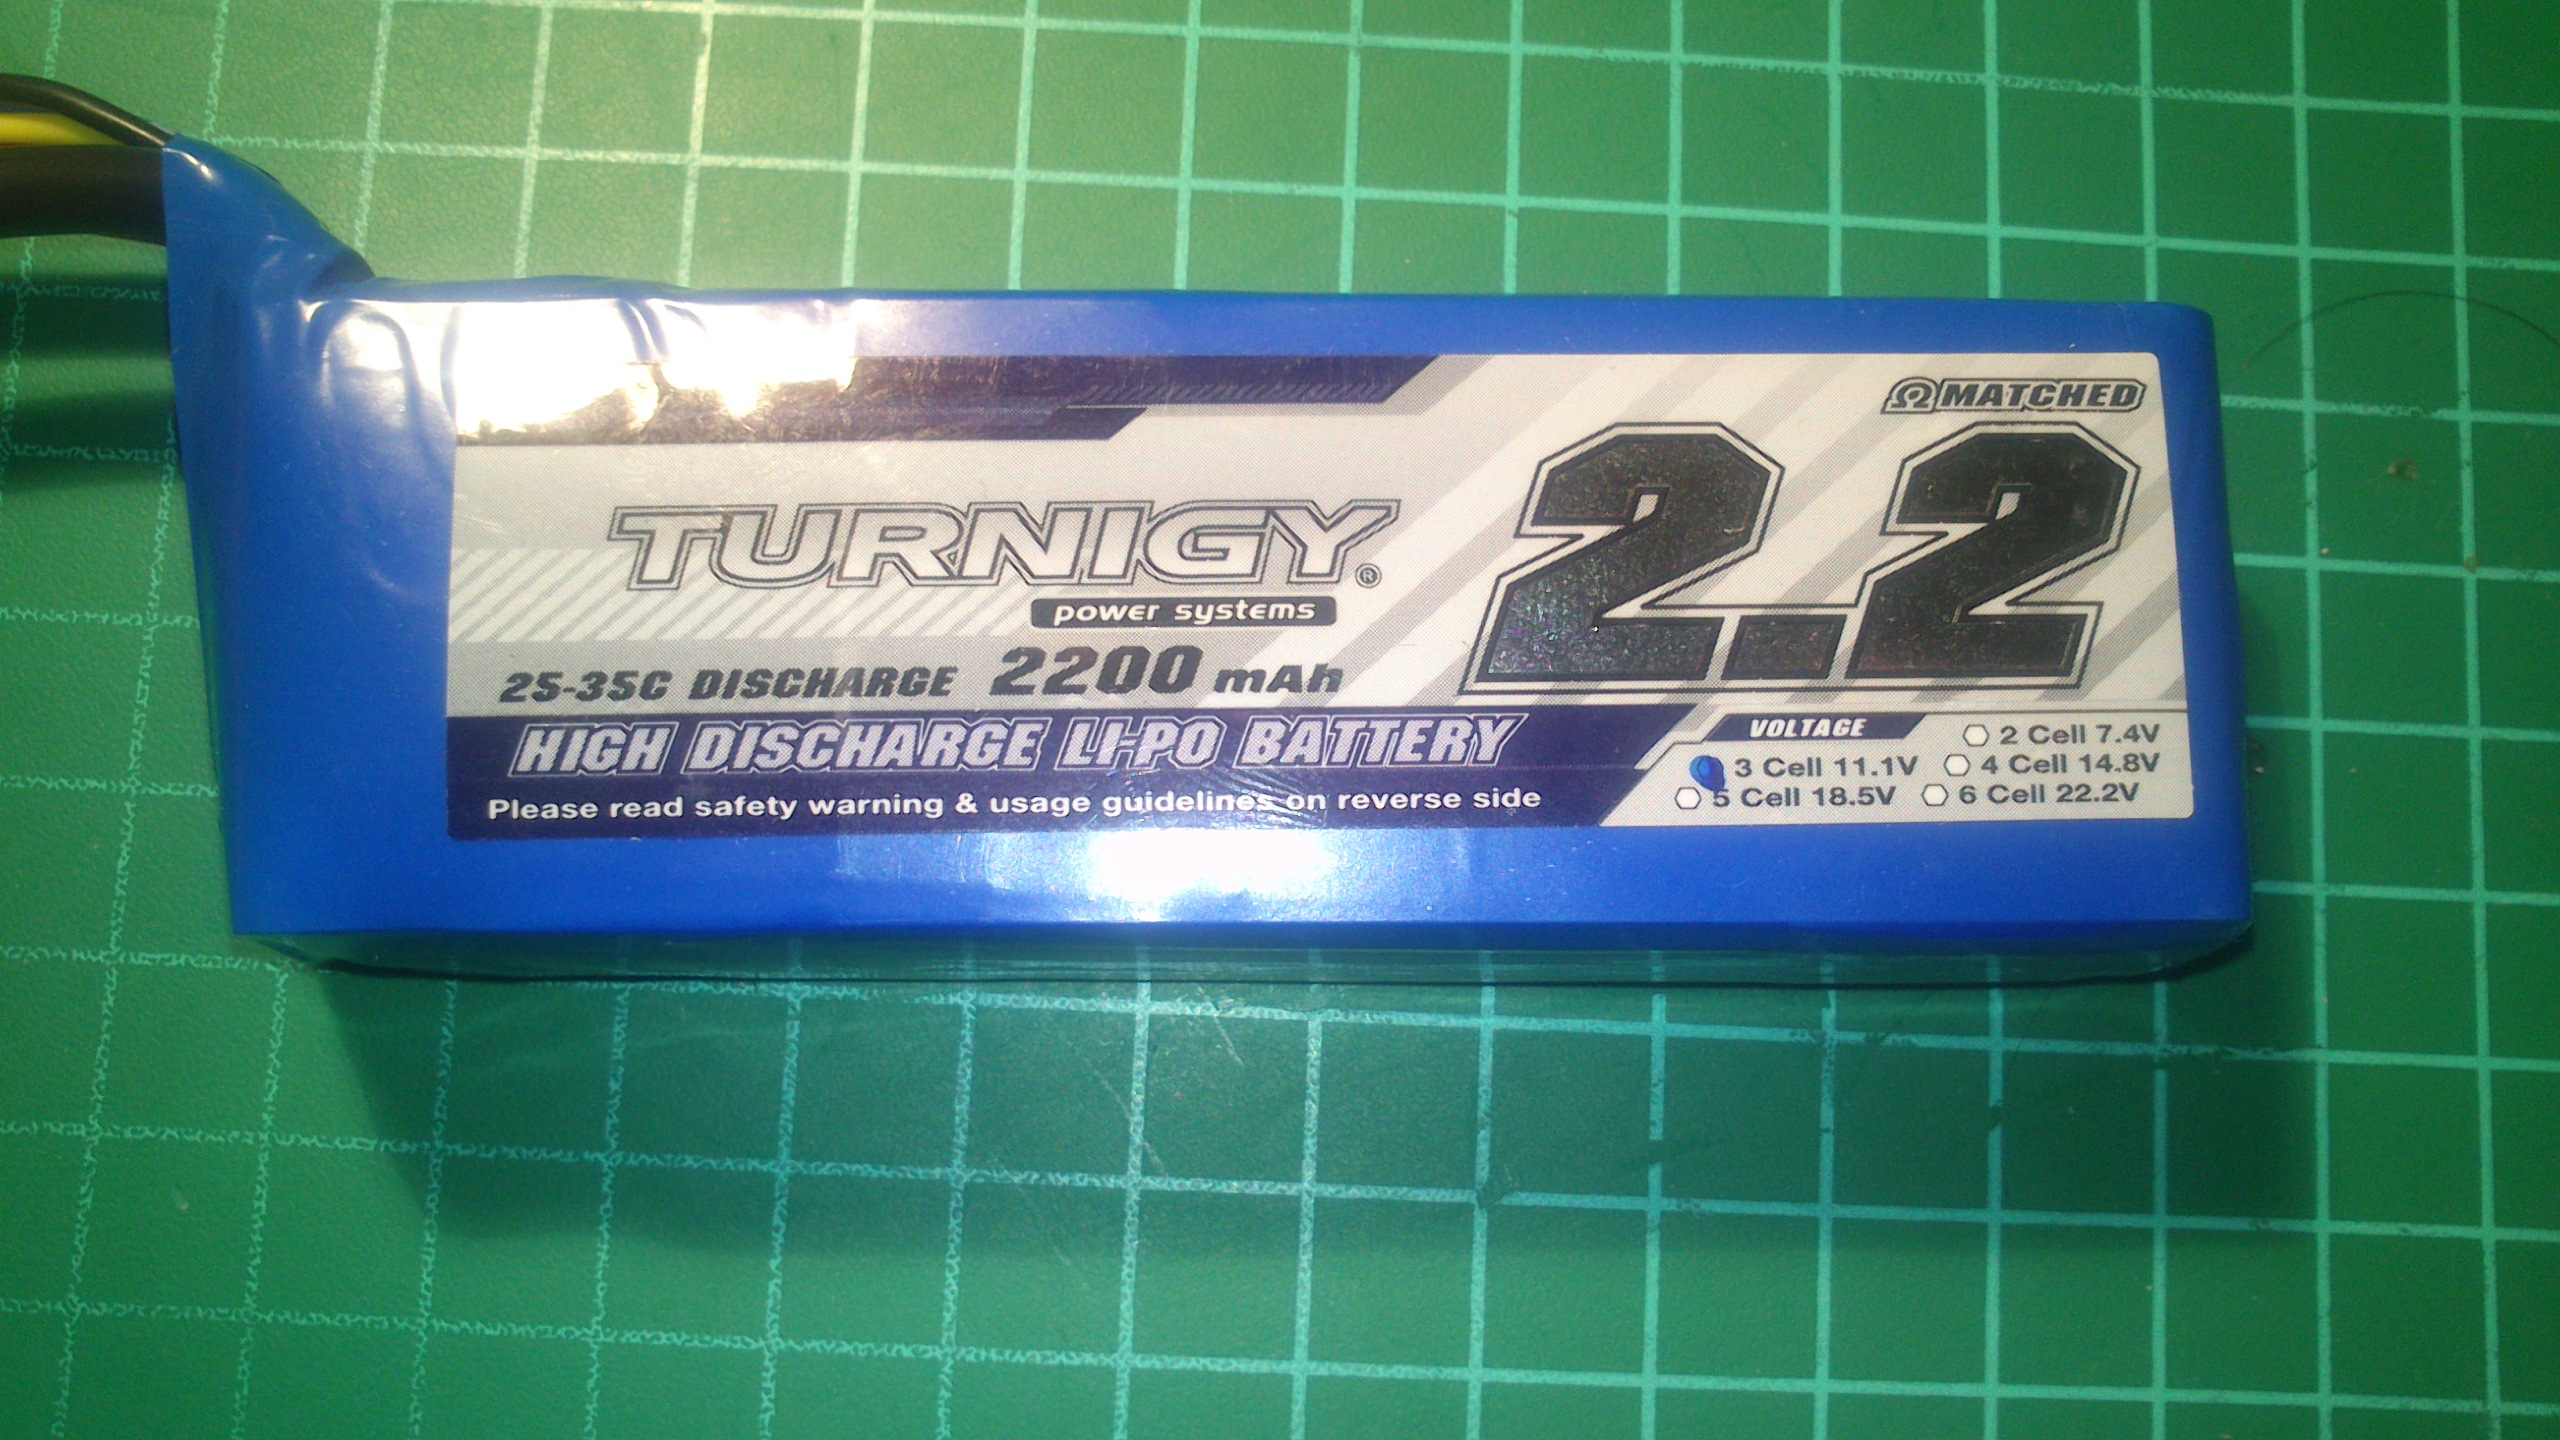
\includegraphics[scale=0.1,viewport=0 400 2560 1250,clip]{images/LiPo.jpg} \\
\end{center}
El conector de càrrega és el $JST-XH$ i el de descàrrega el $XT60$. Per a tenir en compte amb per al quadcopter és interessant saber que pesa $188g$ i respecte a l'estructura (frame) que les seves dimensions són de $105x33x24mm$.

\subsubsection*{Regulador Step-Down}
Per adaptar la tensió de 11.1V de la bateria LiPo a 5V per alimentar la Raspberry Pi, és necessari un regulador. En aquest cas es té l'Interruptor-Mode Màxim BEC LM2576S, que proporciona fins a 3A de corrent \\
\begin{center}
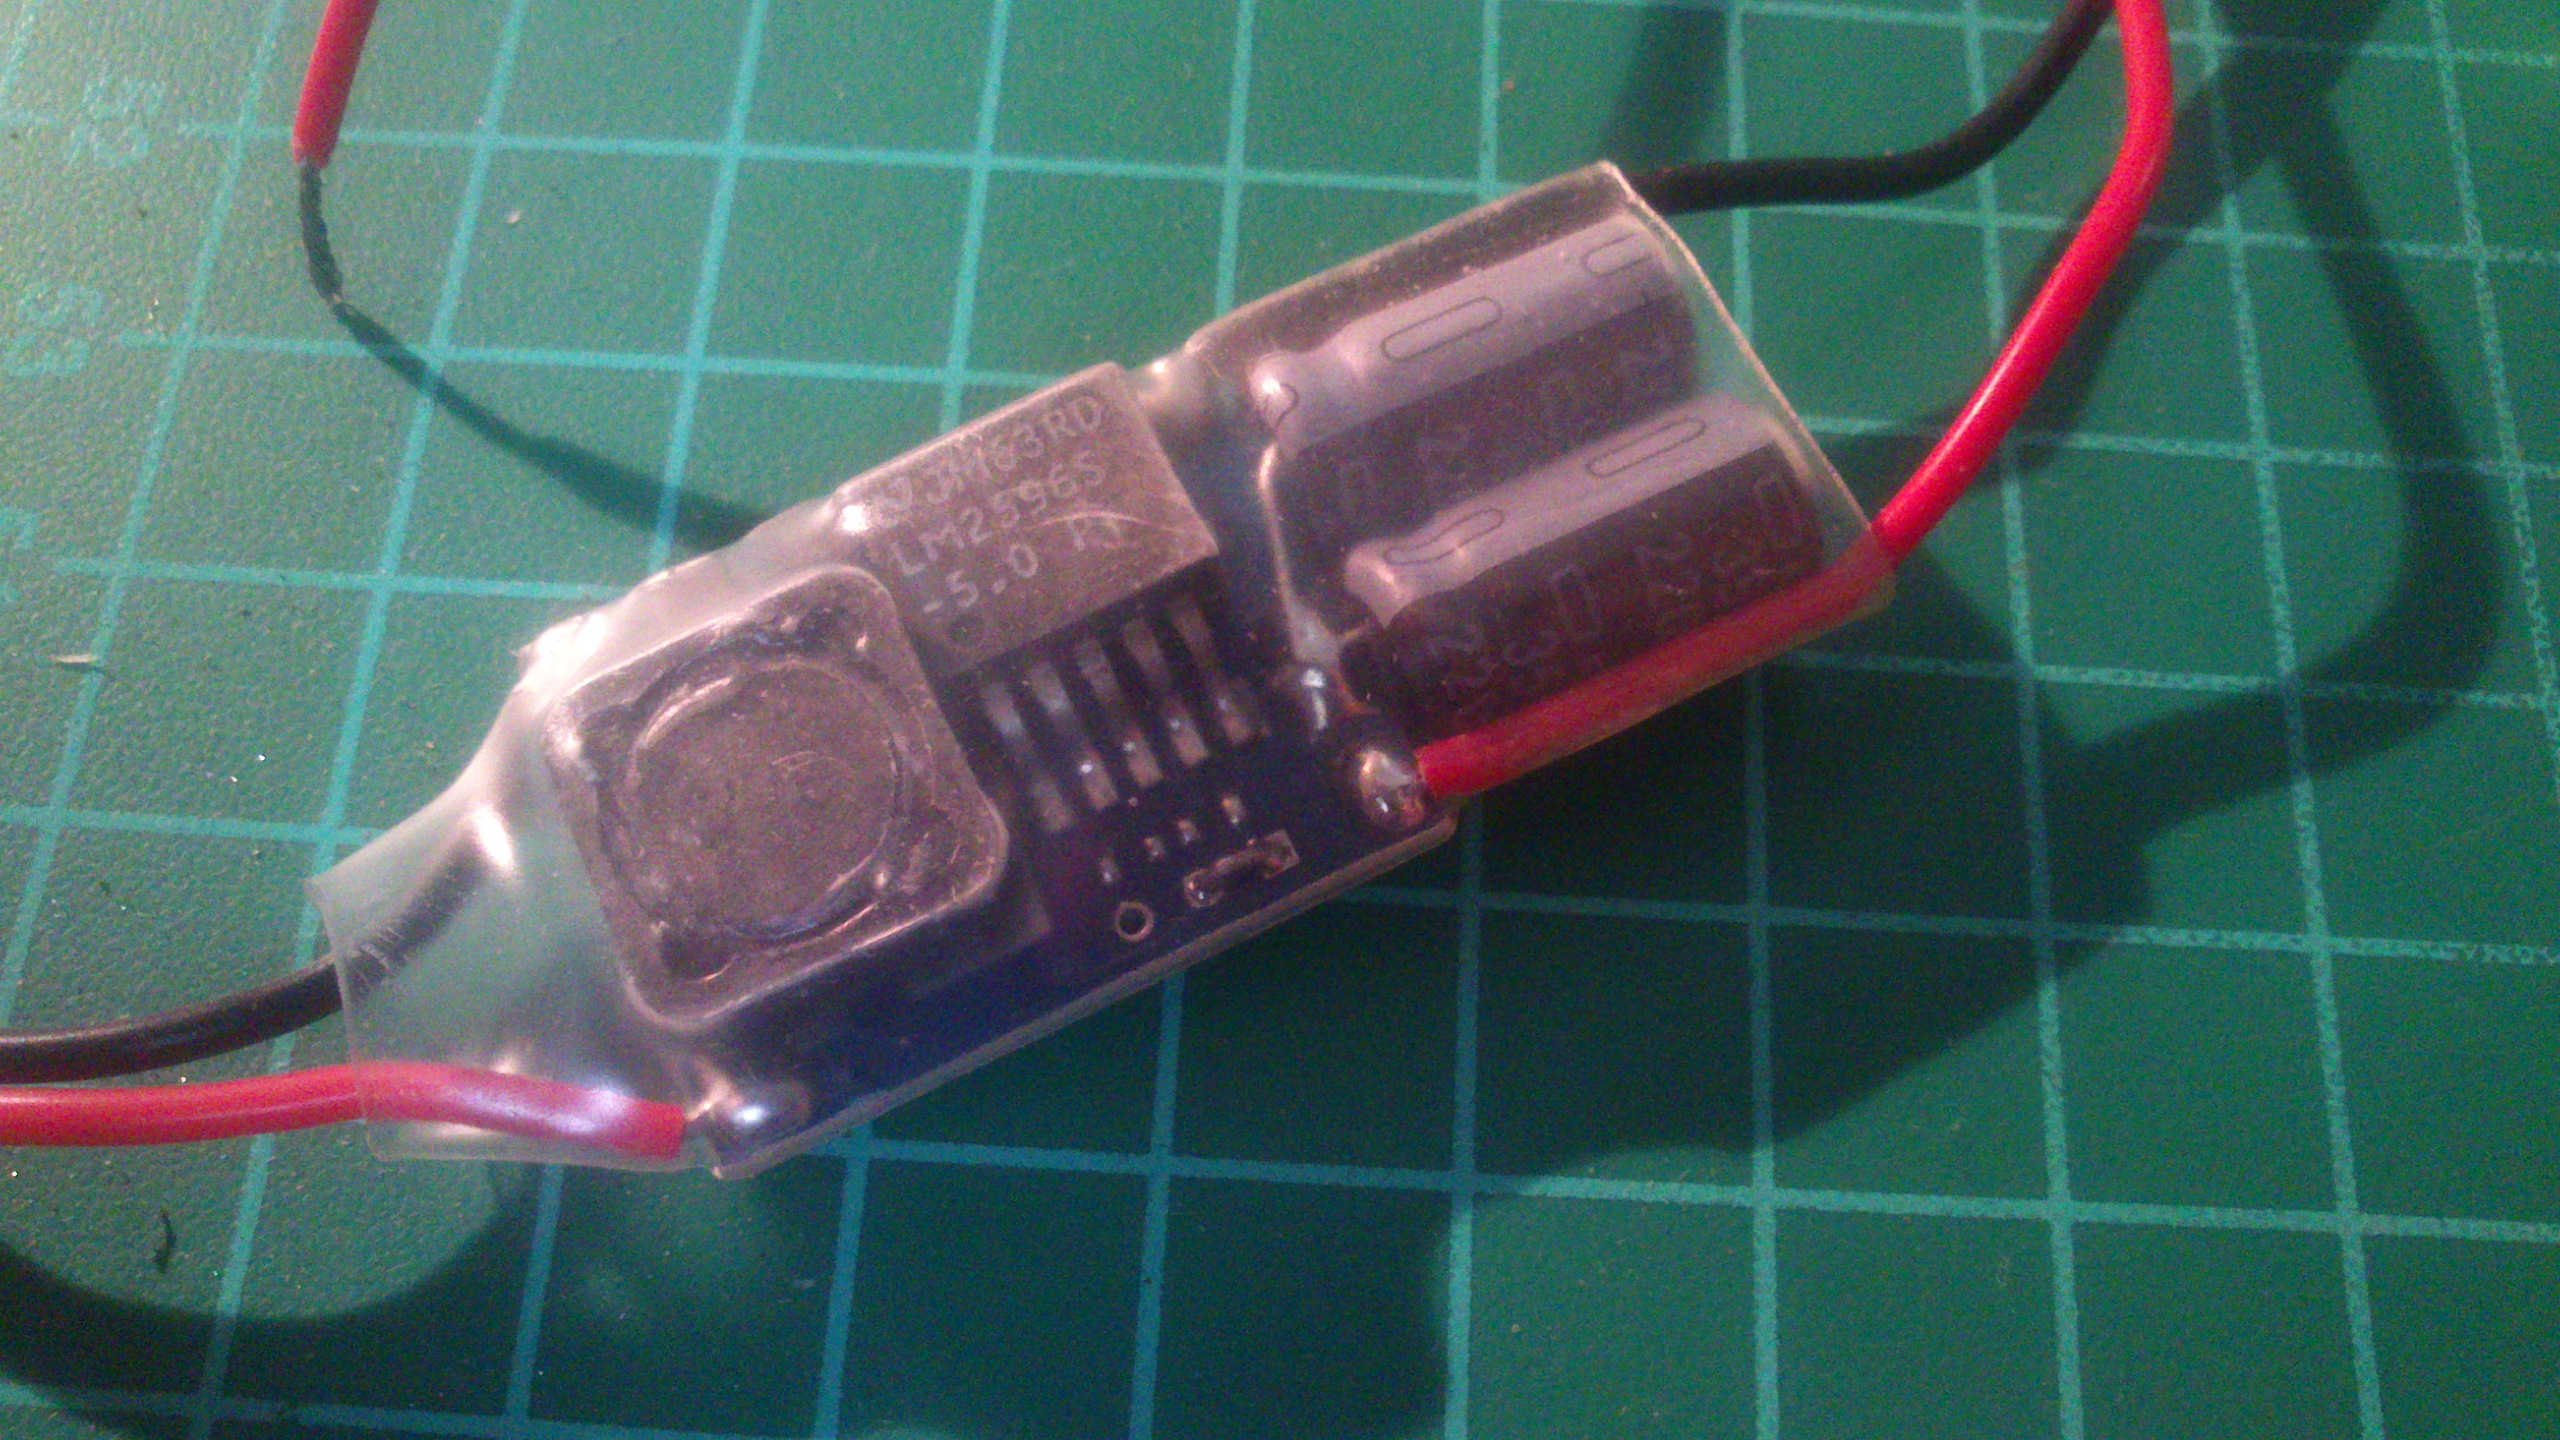
\includegraphics[scale=0.06]{images/Reg_stepdown.jpg}
\end{center}

L'esquema del component \cite{lm2576s}:

\begin{center}
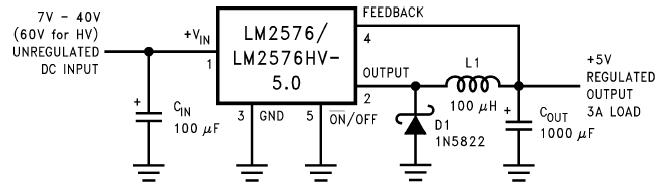
\includegraphics[scale=0.55]{images/lm2576s.jpeg} 
\end{center}

\subsubsection*{Motors Brushless}
Els actuadors que s'utilitzen són motors brushless (BL-DC). En partircular el Turnigy 2213 20turn 1050kv 19A Outrunner. Les seves especificacions més rellevants són:
\begin{itemize}
\item Kv: 1050rpm/v
\item Corrent de treball: 6A ~ 16A
\item Corrent de pic: 19A
\item Pes: 56g
\item Dimensions: 27.6 x 32mm
\item Mida de l'eix: 3.175mm
\end{itemize}
La relació entre la senyal de PWM i la força, així com el consum es troben a l'Annex
\subsubsection*{Variador ESC}

Per a controlar un motor brushless l'etapa de potència a utilitzar un ESC (Electronic Speed Controller) que és un  variador que consta d'un inversor trifàsic:
\begin{center}
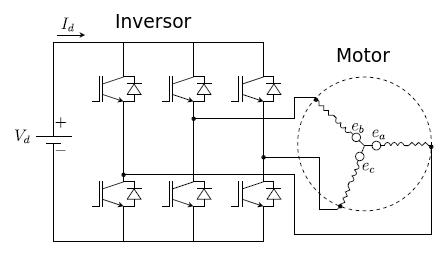
\includegraphics[scale=0.4]{images/ESC.jpeg}
\end{center}

Turnigy AE-20A Brushless ESC
Specification:
Output:  Continuous 20A, burst 25A up to 10 seconds.
Input Voltage:  2-4 cells lithium battery or 5-12 cells NIMH battery.   
BEC:  Linear 2A @ 5V
Control Signal Transmission: Optically coupled system.
Max Speed:     
   2 Pole: 210,000rpm
   6 Pole: 70,000rpm
   12 Pole: 35,000rpm
Size:  50mm (L) * 26mm (W) * 12mm (H).
Weight:  19g.

Features:
High performance microprocessor brings out the best compatibility with all kinds of motors and the highest driving efficiency.
Wide-open heatsink design to get the best heat dissipation effect.
Improved Normal, Soft, Very-Soft start modes, compatible with aircraft and helicopter. 
Smooth, linear, quick and precise throttle response.
Multiple protection features: Low-voltage cut-off protection / Over-heat protection / Throttle signal loss protection
Programable via transmitter
Programming features:
Brake setting (we recommend using brake for only folding props applications)
Battery type(Li-xx or Ni-xx) 
Low voltage cutoff setting 
Factory default setup restore 
Timing settings (to enhance ESC efficiency and smoothness) 
Soft acceleration start ups (for delicate gearbox applications)
Low voltage cutoff type (power reduction orirnmediate shutdown)
 
Factory default settings:
Brake:  off 
Battery type:  Li-xx (Li-ion or Li-Po) 
Low voltage cutoff threshold:  Soft cut-off (2.6V) 
Timing setup:  Low 
Soft Acceleration Start Up:  Normal \\
Low voltage cutoff type:  Medium


\subsubsection*{Frame}
Peso 190g

\subsubsection*{Hèlix}


\newpage
\subsection{Muntatge}
% Descripción del procedimiento por pasos y con fotos

\begin{center}
\begin{tikzpicture}
%%% POWER LINES
\path[draw] (1,8.25) node {\large 12V};
\path[draw] (2,8.25) node {\large 0V};
\path[draw,line width=6pt,color=red,o-o] (1,1) -- (1,8);
\path[draw,line width=6pt,color=black,o-o] (2,1) -- (2,8);

%%% LIPO LEVEL
\path[draw,line width=2pt,color=red] (1,6) -- (3,6);
\path[draw,line width=2pt,color=black] (2,5.5) -- (3,5.5);
\path[draw] (3.8,5.75) node[draw,line width=3pt] (nodeA) {\huge LiPo};
\path[draw] (7.2, 5.75) node[draw,line width=3pt] (nodeA) {\huge IMU};
\path[draw,line width=2pt,color=olive] (7.2,5.35) -- (7.2,4.6);
\path[draw] (7.6,5) node (nodeC) { I2C};
\path[draw] (9.8, 5.75) node[draw,line width=3pt] (nodeA) {\huge Rec.};
\path[draw, line width=2pt,color=green] (9.8, 5.34) -- (9.8, 4.5) -- (7.95, 4.5);
\path[draw] (9, 4.8) node {5xCHNL};
\path[draw,line width=2pt,dotted, color=cyan](10.6,5.75) -- (12.3,5.75);
\path[draw] (13, 5.75) node[draw,line width=3pt] (nodeA) {\huge Em.};

%%% BUCK LEVEL
\path[draw,line width=2pt,color=red] (1,4.5) -- (3,4.5);
\path[draw,line width=2pt,color=black] (2,4) -- (3,4);
\path[draw] (4.1,4.25) node[draw,line width=3pt] (nodeA) {\huge BUCK};
\path[draw,line width=2pt,color=red] (5.26,4.5) -- (6.5,4.5);
\path[draw,line width=2pt,color=black] (5.2,4) -- (6.5,4);
\path[draw] (7.2,4.25) node[draw,line width=3pt] (nodeA) {\huge RPi};
\path[draw] (5.8,4.8) node (nodeC) {5V};
\path[draw, line width=2pt, color=green] (7.95,4)--(9.8,4) -- (9.8,3.2);
\path[draw] (9.2,3.65) node {PWM};

%%% ESC LEVEL
\path[draw, line width=2pt, color=red] (1,3) -- (9,3);
\path[draw, line width=2pt, color=black] (2,2.5) -- (9,2.5);
\path[draw] (9.8,2.75) node[draw,line width=3pt] (nodeC) {\huge ESC};
\path[draw] (10.3,2.1) node (nodeC) {\large (x4)};
\path[draw, line width=2pt, color=blue] (10.6,3) -- (12,3);
\path[draw, line width=2pt, color=blue] (10.6,2.75) -- (12,2.75);
\path[draw, line width=2pt, color=blue] (10.6,2.5) -- (12,2.5);
\path[draw] (13,2.75) node[draw,line width=3pt] (nodeC) {\huge Motor};
\path[draw] (13.7,2.1) node (nodeC) {\large (x4)};
\end{tikzpicture}
\end{center}

% \section{Generació de la consigna}
% Descripcion general de como se genera, envia y procesa la consigna
% Imagen con esquema
% \subsection{Configuració de la RPi com a Access Point}
% Describir procedimiento de configuración de la RPi para ser AP
% \subsection{Aplicació d'Android }
% Explicar que la App es en java y para Android y que envia la informacion a la RPi (configurada como AccessPoint).
% Dar el codigo de la aplicacion

% \section{Comparació amb un control PID}

\newpage
\section{Anàlisi econòmic}

\newpage
\section*{ANNEXES}
\subsection*{Annex 1: Obtenció vector de forces}
Per a treballar amb la dinàmica del sistema s'obté el vector de forces a partir del Lagrangià:
\begin{verbatim}
clear all
clc

%%% Para usar la funcion Laplace en el archivo Laplace.m se deben declarar
%%% las variables de esta manera:

syms x dx ddx y dy ddy z dz ddz Phi dPhi ddPhi Theta dTheta ddTheta Psi dPsi ddPsi
syms f1 f2 f3 f4 m1 m2 m3 m4
% syms w1 w2 w3 w4
syms Ixx Iyy Izz
syms Ax Ay Az               % No se tienen en cuenta coeficientes de friccion
syms k m g l b

l=0.165             % longitud de los brazos
Ixx=0.004           % Momento de inercia del eje x 
Iyy=0.004           % Momento de Inercia del eje y
Izz=0.008           % Momento de Inercia del eje z
m=0.85              % Peso del Quadcopter
g=9.81              % gravedad 

%%% El vector de variables que se usaran

v=[x dx ddx y dy ddy z dz ddz Phi dPhi ddPhi Theta dTheta ddTheta Psi dPsi ddPsi]

Xi=[x; y; z]
dXi=[dx; dy; dz]

Eta=[Phi; Theta; Psi]
dEta=[dPhi; dTheta; dPsi]

Q=[Xi; Eta]
dQ=[dXi; dEta]

II=[[Ixx 0 0];
    [0 Iyy 0];
    [0 0 Izz]]

A=[[Ax 0 0];
   [0 Ay 0];
   [0 0 Az]]   
   
R=[[cos(Psi)*cos(Theta) cos(Psi)*sin(Theta)*sin(Phi)-sin(Psi)*cos(Phi) cos(Psi)*sin(Theta)*cos(Phi)+sin(Psi)*sin(Phi)];
    [sin(Psi)*cos(Theta) sin(Psi)*sin(Theta)*sin(Phi)+cos(Psi)*cos(Phi) sin(Psi)*sin(Theta)*cos(Phi)-cos(Psi)*sin(Phi)];
    [-sin(Theta) cos(Theta)*sin(Phi) cos(Theta)*cos(Phi)]]

Weta=[[1 0 -sin(Theta)];
      [0 cos(Phi) cos(Theta)*sin(Phi)];
      [0 -sin(Phi) cos(Theta)*cos(Phi)]]
  
J=transpose(Weta)*II*Weta  
  
L=m/2*transpose(dXi)*dXi+(1/2)*transpose(dEta)*transpose(Weta)*II*Weta*dEta-m*g*z

%%% Aqui se obtiene con el Lagrangiano el vector de fuerzas F segun
%%% F=(d/dt)(dp(L)/dp(dq))-d(L)/dq

F=Lagrange(L,v)

%%% Derivando a mano se obtiene que TauB=J*ddEta+CdEta 
%%% Y como TauB=[F(4); F(5); F(6)], se tiene que el termino de Coriolis es:

CdEta=[F(4); F(5); F(6)]-J*[ddPhi; ddTheta; ddPsi]

%%% Hasta se tiene el producto Coriolis(Eta,dEta)*dEta. Pero como matlab
%%% no elimina las aceleraciones se hace a mano, y queda:

CdEta = [(Iyy*dTheta^2*sin(2*Phi))/2 - (Izz*dTheta^2*sin(2*Phi))/2 - Ixx*dPsi*dTheta*cos(Theta) - (Iyy*dPsi^2*sin(2*Phi)*cos(Theta)^2)/2 + (Izz*dPsi^2*sin(2*Phi)*cos(Theta)^2)/2 - Iyy*dPsi*dTheta*cos(2*Phi)*cos(Theta) + Izz*dPsi*dTheta*cos(2*Phi)*cos(Theta);
          dPhi*(Ixx*dPsi*cos(Theta) - 2*Iyy*dTheta*cos(Phi)*sin(Phi) + 2*Izz*dTheta*cos(Phi)*sin(Phi) + Iyy*dPsi*cos(Phi)^2*cos(Theta) - Izz*dPsi*cos(Phi)^2*cos(Theta) - Iyy*dPsi*cos(Theta)*sin(Phi)^2 + Izz*dPsi*cos(Theta)*sin(Phi)^2)  - Ixx*dPsi^2*cos(Theta)*sin(Theta) + Iyy*dPsi^2*cos(Theta)*sin(Phi)^2*sin(Theta)  + Izz*dPsi^2*cos(Phi)^2*cos(Theta)*sin(Theta);
          -dPhi*(Ixx*dTheta*cos(Theta) - Iyy*dTheta*cos(Phi)^2*cos(Theta) + Izz*dTheta*cos(Phi)^2*cos(Theta) + Iyy*dTheta*cos(Theta)*sin(Phi)^2 - Izz*dTheta*cos(Theta)*sin(Phi)^2 - 2*Iyy*dPsi*cos(Phi)*cos(Theta)^2*sin(Phi) + 2*Izz*dPsi*cos(Phi)*cos(Theta)^2*sin(Phi)) - Iyy*dTheta^2*cos(Phi)*sin(Phi)*sin(Theta) + Izz*dTheta^2*cos(Phi)*sin(Phi)*sin(Theta) + 2*Ixx*dPsi*dTheta*cos(Theta)*sin(Theta) - 2*Izz*dPsi*dTheta*cos(Phi)^2*cos(Theta)*sin(Theta) - 2*Iyy*dPsi*dTheta*cos(Theta)*sin(Phi)^2*sin(Theta)]
      
T=f1+f2+f3+f4               % Fuerza total (Total Thrust)
TB=[0; 0; T]                % Thrust en la referencia del Quadctopter
TauB=[l*(f4-f2);
      l*(f3-f1);
      % (m1+m2+m3+m4)]
      b*(f1-f2+f3-f4)]
\end{verbatim}
\newpage

%\begin{lstlisting}

%\end{lstlisting}

\subsection*{Annex 2:Preparació de la Raspberry Pi}
Per a posar a punt la RPi s'ha d'instal·lar Raspbian i configurar-lo per tal que es pugui comunicar amb la placa MPU-6050.
\subsubsection*{Instalació Raspbian}
Havent introduït la targeta SD en un lector adeqüat, es detecta en una terminal mitjançant l'ordre \textit{df -h}. Suposant que hagués estat gravada anteriorment:
\begin{center}
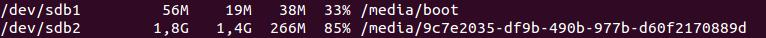
\includegraphics[scale=0.7]{images/InstalRasp1.jpeg}
\end{center}
S'han de desmontar les dos particions, tant la \textit{/dev/sdb1} com la \textit{/dev/sdb2}:
\begin{verbatim}
           umount /dev/sdb1
           umount /dev/sdb2
\end{verbatim}
Havent descarregat la imatge a instalar per exemple a l'Escriptori, es procedeix amb:
\begin{verbatim}
    sudo dd bs=4M if=~/Escritorio/2013-07-26-wheezy-raspbian.img of=/dev/sdb
\end{verbatim}
Passats uns minuts ja es té la SD grabada amb el sistema operatiu Raspbian.
\subsubsection*{Configuració de la Raspberry}
Per tal de poder comunicar la RPi amb la IMU MPU-6050 per I2C és necessari configurar el sistema. Primer és necessari instal·lar els drivers més rellevants. De l'arxiu
\begin{verbatim}
           sudo nano /etc/modules
\end{verbatim}
s'han d'afegir les següents dues línies al final de l'arxiu:
\begin{verbatim}
           i2c-bcm2708
           i2c-dev
\end{verbatim}
En l'arxiu blacklist:
\begin{verbatim}
           sudo vi /etc/modprobe.d/raspi-blacklist.conf
\end{verbatim}
les següents dues línies han de començar amb un signe \# (de comentari):
\begin{verbatim}
           #blacklist spi-bcm2708
           #blacklist i2c-bcm2708
\end{verbatim}
Per provar de connectar el sensor, és necessari seguir primer el connexionat:

\begin{figure}[h!]
\begin{center}
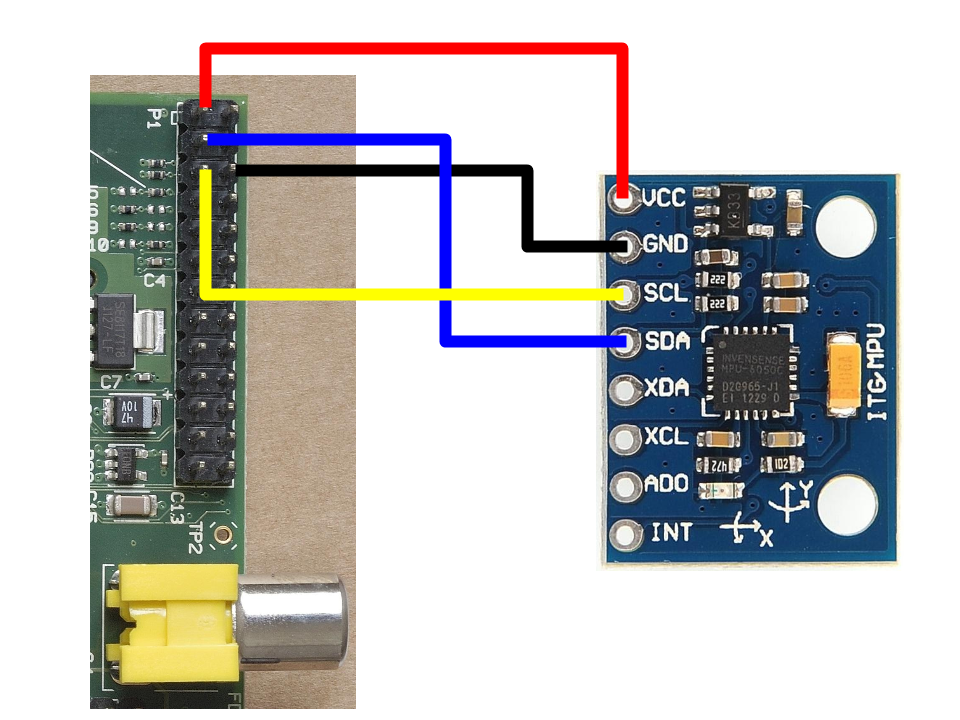
\includegraphics[scale=0.2,viewport=0 200 800 720,clip]{images/ConSens.jpg}
\caption{Connexió per I2C entre MPU-6050 i RPi}
\end{center}
\end{figure}


És a dir:
\begin{itemize}
\item Pin1-3.3V es connecta VCC.
\item Pin3-SDA es connecta a SDA
\item Pin5-SCL es connecta a SCL
\item Pin6-Ground es connecta a GND
\end{itemize} 
S'ha d'instal·lar el paquet $i2c-tools$:
\begin{verbatim}
           sudo apt-get install i2c-tools
\end{verbatim}
Per a veure el sensor s'escriu:
\begin{verbatim}
           sudo i2cdetect -y 1
\end{verbatim}
El resultat és 

\begin{figure}[h!]
\begin{center}
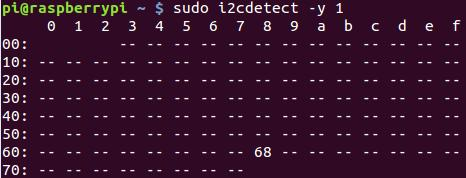
\includegraphics[scale=0.7]{images/i2cdetect.jpg}
\caption{Detecció del sensor MPU-6050}
\end{center}
\end{figure}
que és el dispositiu que correspon al MPU-6050.

\subsubsection*{Llibrería wiringPi}
S'utilitza aquesta llibrería\cite{wiringPi} com a interfície del GPIO (General Porpouse Input Output). Permet, per tant,llegir tant les consignes com els sensors i generar les accions de control. 
La instal·lació i descripció de la llibrería està explicat a la pàgina web incluída a la bibliografía.

\newpage
\subsection*{Annex 3: Filtre de kalman}
\newpage
\subsection*{Annex 4: Caracterització dels motors}
Per tal de poder controlar la planta és necessari saber còm responen els actuadors per tal de realitzar un control precís. D'aquests és necessari saber quina força i moment proporcionen, així com el consum d'energia donat un PWM. 
Per a obtenir una corva de la força respecte del PWM es pesa amb una balança l'acció del motor. La rudimentària bancada que es té per a tal objectiu és d'un colze articulat a un eix de tal manera que la distància de l'eix del motor al fulcre i d'aquest a la balança sigui la mateixa (en aquest cas de 12 cm):

\begin{figure}[h!]
\begin{center}
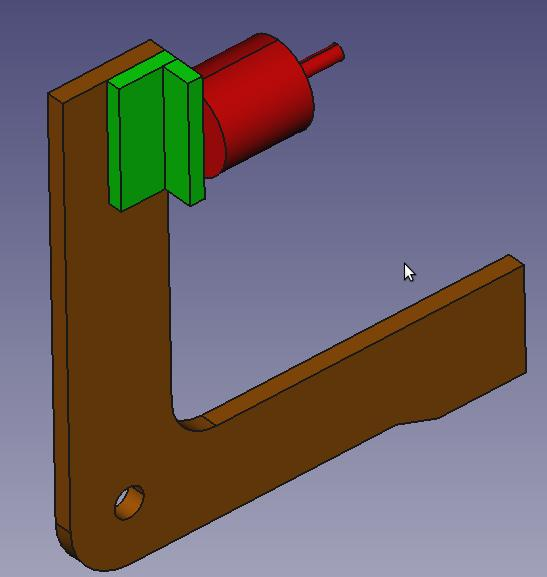
\includegraphics[scale=0.4]{images/bancada1.jpeg}
\caption{Bancada per a l'estudi del motor}
\end{center}
\end{figure}
Les parts estan fetes de fusta (part marró) i plàstic ABS (part verda). Tota l'estructura es subjecta a unes fustes:

\begin{figure}[h!]
\begin{center}
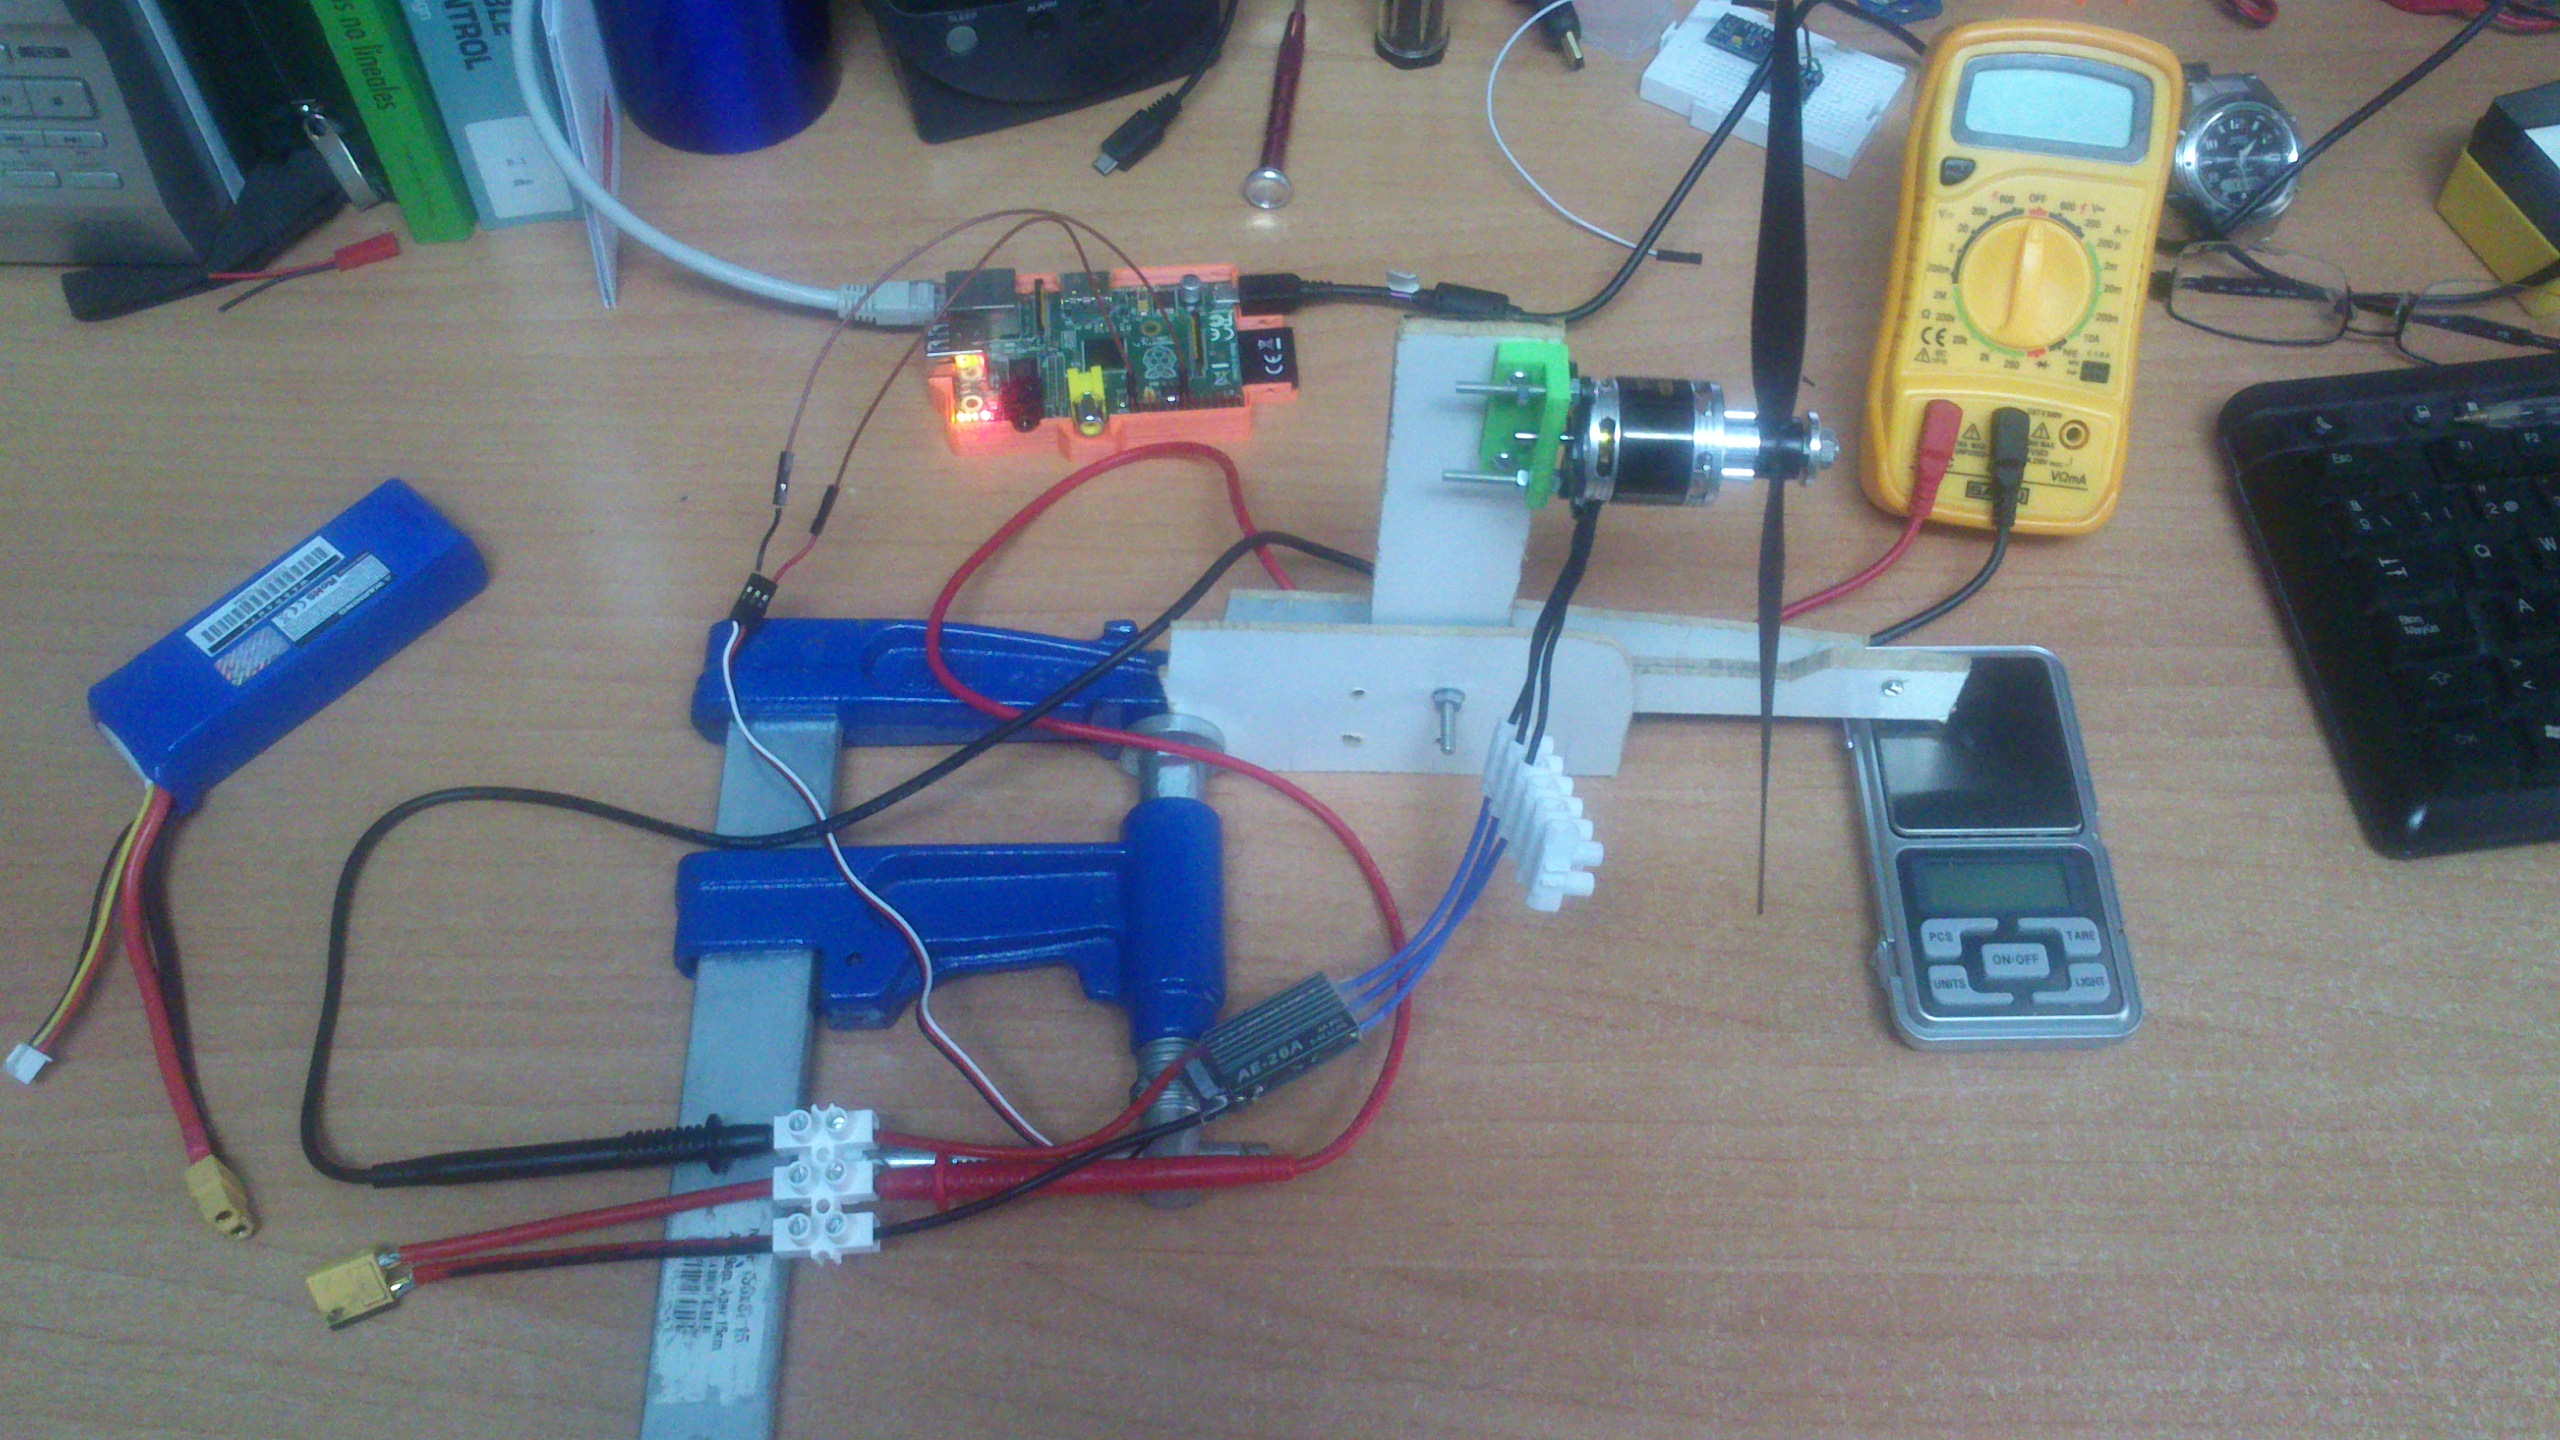
\includegraphics[scale=0.09]{images/montaje.jpg}
\caption{Montatge per a l'estudi del motor}
\end{center}
\end{figure}

Es transmet al ESC a quina velocitat s'ha de fer funcionar al motor des de la Raspberry Pi per mitjà d'una senyal PWM. El programa que s'executa per a fer les proves és:

\begin{verbatim}
#include <stdio.h>
#include <termios.h>
#include <wiringPi.h>
#include <unistd.h>

#define PIN 2 // pin 13

int main(void){

        int i,p;
        wiringPiSetup();

        pinMode(PIN,OUTPUT);
        digitalWrite(PIN,LOW);

        for(i=60;i<=100;i+=5){
                for(p=0;p<250;p++){
                        digitalWrite(PIN,HIGH);
                        delayMicroseconds(950+i*10);
                        digitalWrite(PIN,LOW);
                        delayMicroseconds(19050-i*10);

                        printf("PWM(i): %d \t h:%d \n",i,p);
                }
        }
        return 0;
}
\end{verbatim}

S'obté una mesura de força i d'intensitat per cada increment del 0.25\% del PWM enviat al Variador. Sobté:

\begin{figure}[h!]
\begin{center}
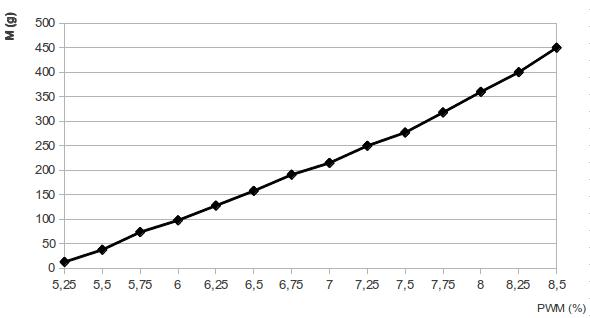
\includegraphics[scale=0.8]{images/MvsPWM.jpeg}
\caption{Relació entre la força (en grams) i el PWM}
\end{center}
\end{figure}
En l'eix de les abscises el PWM(\%) és entre el 5\% i el 10\% de la senyal enviada, que correspon al mínim i màxim que el motor. Com que per a un PWM elevat la força era massa gran i no es preveu que es farà funcionar el sistema en semblants condicions de treball, no s'estudia. 

Es veu una relació proporcional del PWM amb la força generada. Es considera que una regressió lineal serà suficient. S'obté que la força $f(PWM)$ del motor serà:
$$f=32.5758 \cdot PWM(\%)-32.1758$$
amb un coeficient de determinació en la regressió és de  $R^2=0.9929$. Aquest resultat facilita el problema en ser una relació prou senzilla.

Per a l'intensitat es té una relació tan amigable com en el cas anterior, però com que no serà cas d'estudi, només es veurà una aproximació del que pot arribar a consumir cada motor per a assegurar una autonomía de vol no irrisòria. Es té que 
\newpage
\begin{figure}[!h]
\begin{center}
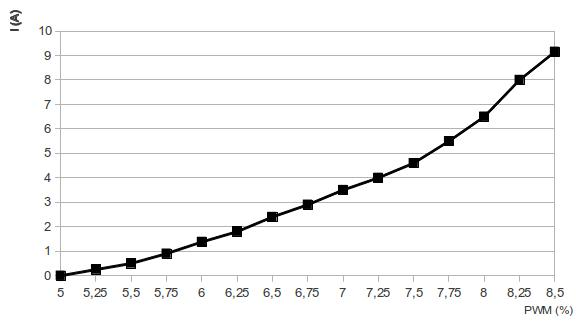
\includegraphics[scale=0.8]{images/IvsPWM.jpeg}
\caption{Relació entre la força (en grams) i el PWM}
\end{center}
\end{figure}

Com que en el punt d'equilibri cada motor suporta una cuarta part del pes, el PWM hauría de correspondre a una força de $m_{Quadcopter}\cdot g/4\approx0.225$kg. El consum corresponent és de $3.5$A aproximadament. Entre els quatre motors es consumiràn $3.5 \cdot 4=14$A. Com que la bateria es de 2200mAh es suposa una autonomia de 7 minuts aproximadament. 

\newpage
\begin{thebibliography}{99}
\bibitem{QuadPaper} Teppo Luukkonen (August 22,2011). \textit{Modelling and control of quadcopter}
\bibitem{RPiWiki} Wikipedia de la Raspberry Pi: \url{http://en.wikipedia.org/wiki/Raspberry_Pi}
\bibitem{IMUArduino} Accel·leròmetre i Giròscop MPU-6050 per a Arduino: \url{http://playground.arduino.cc/Main/MPU-6050#.UzhsVCK9jb4}
\bibitem{6050Esp} MPU-6050. Especificació del producte: \url{http://www.invensense.com/mems/gyro/documents/PS-MPU-6000A-00v3.4.pdf}
\bibitem{6050RegMap} MPU-6050. Mapa de Registres i descripcions: \url{http://www.invensense.com/mems/gyro/documents/RM-MPU-6000A-00v4.2.pdf}
\bibitem{lm2576s} LM2576S Datasheet: \url{http://www.ti.com/lit/ds/symlink/lm2576.pdf}
\bibitem{wiringPi} Llibrería wiringPi: \url{http://wiringpi.com/}
\end{thebibliography}{}
\end{document}